% Template:     Informe LaTeX
% Documento:    Archivo de ejemplo
% Versión:      8.3.5 (12/04/2024)
% Codificación: UTF-8
%
% Autor: Pablo Pizarro R.
%        pablo@ppizarror.com
%
% Manual template: [https://latex.ppizarror.com/informe]
% Licencia MIT:    [https://opensource.org/licenses/MIT]

% ------------------------------------------------------------------------------
% NUEVA SECCIÓN
% ------------------------------------------------------------------------------
% Las secciones se inician con \section, si se quiere una sección sin número se
% pueden usar las funciones \sectionanum (sección sin número) o la función
% \sectionanumnoi para crear el mismo título sin numerar y sin aparecer en el índice

\section{Inicio}

\subsection{Introducción}

Año tras año la demanda de energía eléctrica mundial en general va en aumento, lo cual crea la necesidad de disponer de la energía eléctrica suficiente para satisfacer las demandas de consumo. Tanto o más importante como la producción energética, es lograr un máximo aprovechamiento de ésta mejorando el rendimiento de los equipos y de los propios receptores o instalaciones que consumen energía.

\subsection{Objetivo}

Dado que los paneles fotovoltaicos no entregan una potencia constante, ni corriente contante, ni tensión constante, hace falta un circuito que pueda manejarse bien dentro de ciertas variaciones.

El objetivo de este trabajo es, de entre todas las tecnologías y topologías de convertidores electrónicos, seleccionar la más apropiada, que pueda funcionar adaptándose a las variaciones de los paneles fotovoltaicos, y que sea la más eficiente para campos fotovoltaicos de alrededor de 5 kWp y quede dispuesta para que otro convertidor la inyecte a red o utilizar en DC. 

\subsection{Justificación}

En los últimos años se ha despertado un creciente interés por el estudio de los problemas que afectan a la red eléctrica y que degradan la calidad del suministro que reciben los usuarios de la misma. La problemática es muy variada dando lugar a un amplio campo de estudio que, entre otros muchos temas incluye los efectos de la creciente deslocalización de los sistemas de generación, debido a la gran expansión de las energías renovables, y el desarrollo de equipos de compensación activa para la mejora de la calidad del suministro y el ahorro energético.

En este informe se desarrolla el caso del convertidor semi puente boost compacto, adjunto en la \hyperref[fig:topologiareferencia]{figura 1}.

\begin{figure}
	\centering
	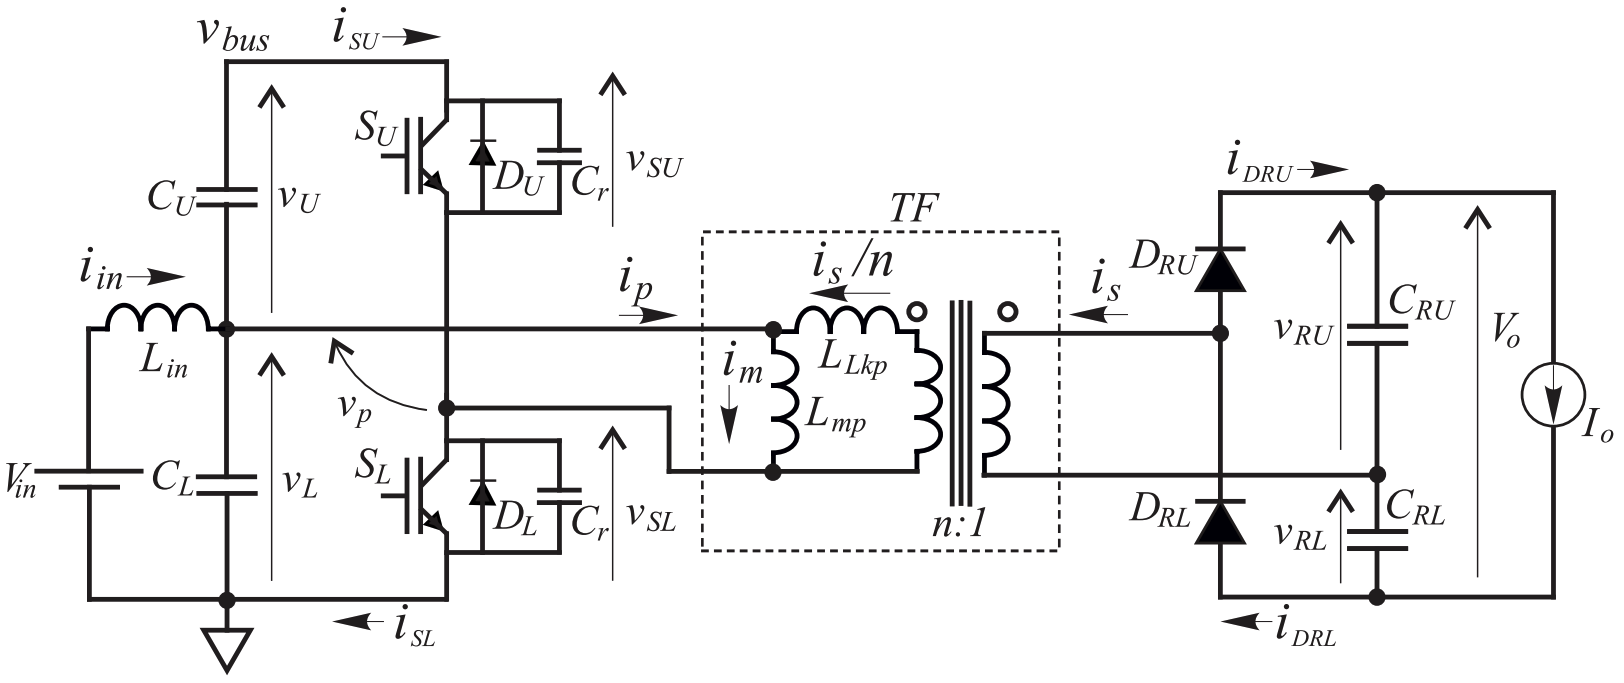
\includegraphics[width=0.9\linewidth]{img/topologiaReferencia}
	\caption[]{Convertidor semipuente boost compacto.}
	\label{fig:topologiareferencia}
\end{figure}

\subsection{Requerimientos de diseño}

\begin{itemize}
	\item Tensión de entrada: $48 \ V_{DC}$
	\item Tensión de salida: $400 \ V_{DC}$
	\item Rango de corriente: $0-40 \ A$
	\item Se pueden colocar módulos DC-DC en paralelo.
\end{itemize}

\clearpage


\section{Marco teórico}

\subsection{Descripción general}

A la entrada del convertidor se conectan los paneles solares, modelados a través de una fuente de tensión constante $V_{in}$. El inductor de entrada se usa para atenuar el ripple en la corriente de entrada $i_{in}$. Dependiendo del requerimiento de ripple en la corriente de entrada, o de la impedancia de salida de la fuente de alimentación es posible eliminar o despreciar el efecto del inductor $L_{in}$. Se usa un transformador de elevador que permita obtener la tensión de salida deseada para el requerimiento de diseño, partiendo de la alimentación a utilizar. Es posible también utilizarlo en una relación $1:1$ si simplemente es necesario un aislamiento. Es posible modelar también el transformador con su inductancia de dispersión $L_{LKp}$ y su inductancia de magnetización $L_{mp}$ referidas al primario.

Se une uno de los bornes del devanado primario del transformador con el nodo entre los capacitores de entrada $C_U$ y $C_L$, siendo que su tensión respecto de tierra es como una fuente de alimentación obtenida a partir de la carga del capacitor $C_L$ y valor $v_L$.  Se tiene una rama con transistores IGBT, formada por un dispositivo superior y otro inferior. Se tienen diodos de recuperación inversa en ambas, que pueden ser los incluidos dentro del mismo encapsulado. Se trabaja con modulación PWM a una frecuencia de conmutación $f_s=1/T_s$. Es importante dejar un pequeño tiempo muerto antes del encendido de cada uno de los IGBT, de modo de evitar un cortocircuito con la fuente. El otro extremo del transformador se conecta entre los IGBT, y tiene una tensión media $v_{SL}$ con respecto al terminal de tierra, conmutando de esa forma entre $v_{bus}$ y GND.

Se tiene así entonces para la tensión del primario $v_P$:

\begin{itemize}
	\item $v_L$ cuando el IGBT inferior está cerrado.
	\item $-v_U$ cuando el IGBT superior está cerrado.
\end{itemize}

Se tiene la salida del secundario del transformador conectada a un rectificador doblador de tensión con los diodos $D_{RL}$ y $D_{RU}$, y por los capacitores $C_{RU}$ y $C_{RL}$, estos últimos filtran la tensión de salida $V_o$, y brindando de acuerdo a la solicitud de la carga una determinada $I_o$. La energía promedio se extrae del panel solar a través del valor medio de $i_P$ del primario del transformador. Se tiene que el valor promedio $\overline{i}_{in}$ de la corriente de la fuente, igual al promedio $\overline{i}_P$.

Partiendo del ciclo de trabajo, si \( d \), tal que \( 0 < d < 1 \), representa el ciclo de trabajo del interruptor \( S_U \), el valor promedio de la tensión en el punto medio de la pierna durante \( T_s \) está dado por \(\overline{v}_{SL} = d\overline{v}_{bus}\), donde \(\overline{v}_{bus}\) es el valor promedio de \( v_{bus} \) durante \( T_s \). En régimen estacionario, los valores promedios de las caídas de tensión sobre el inductor \( L_{in} \) y sobre la inductancia de magnetización \( L_{mp} \) deben ser cero. Por consiguiente, el valor promedio de la tensión sobre el interruptor \( S_L \) es igual al valor promedio de la tensión sobre el capacitor \( C_L \) y a la tensión de la fuente de alimentación, es decir:

\[
\overline{v}_{SL} = \overline{v}_{CL} = \overline{V}_{\text{in}}
\]

En conjunto con la condición \(\overline{v}_{SL} = d\overline{v}_{bus}\), se implica que:

\[
\overline{v}_{bus} = \frac{V_{in}}{d}
\]

Los capacitores de amortiguación \( C_r \) mitigan el apagado de los interruptores \( S_U \) y \( S_L \), retrasando el incremento de sus correspondientes tensiones \( v_{SU} \) y \( v_{SL} \) durante el apagado.

\begin{figure}
	\centering
	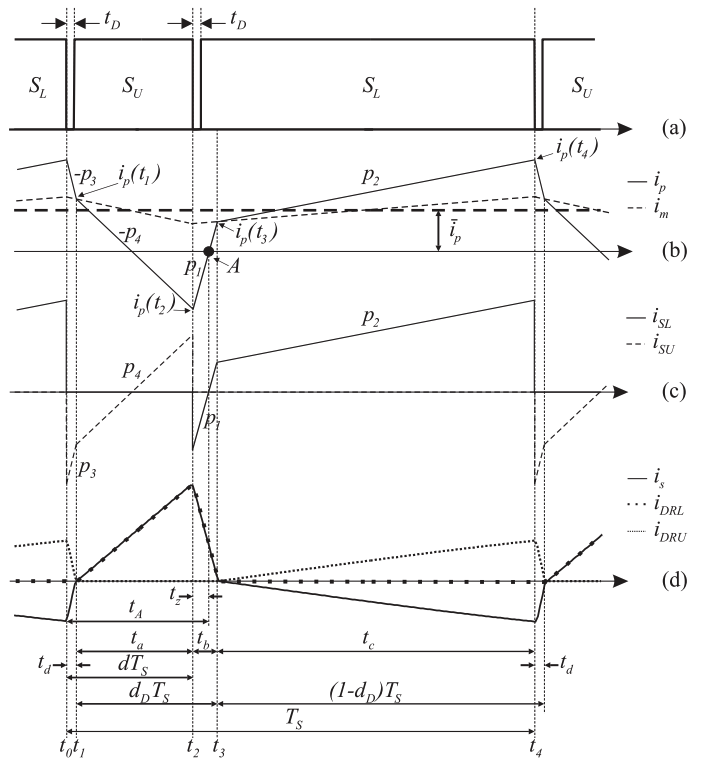
\includegraphics[width=0.7\linewidth]{img/formaOnda1}
	\caption{Formas de onda para \( d \leq 0.5 \): (a) Señales de encendido \( S_U \) y \( S_L \). (b) \( i_p \), \( \overline{i}_p \) e \( i_m \). (c) \( i_{SL} \) e \( i_{SU} \). (d) \( i_s \), \( i_{DRL} \) e \( i_{DRU} \).}
	\label{fig:formaonda1}
\end{figure}

\subsection{Operación}

Para realizar un análisis del comportamiento del convertidor en estado estacionario, se asumirá que los capacitores \( C_L \), \( C_U \), \( C_{RU} \) y \( C_{RL} \) son lo suficientemente grandes como para mantener constante la tensión sobre sus bornes durante un ciclo \( T_s \) de PWM. Por lo tanto, para este análisis, las tensiones \( v_L \) y \( v_U \) serán reemplazadas (a partir de las ecuaciones (3-1) y (3-2)) por fuentes de tensión constante de valor \( V_{in} \) y \( V_U = \frac{V_{in}(1 - d)}{d} \), respectivamente, que corresponden a sus valores medios en estado estacionario. De igual manera, las tensiones \( v_{RU} \) y \( v_{RL} \) serán reemplazadas por las tensiones constantes \( V_{RU} \) y \( V_{RL} \), que corresponden a sus valores medios teóricos en estado estacionario. Además, en este análisis no se considerarán los capacitores de snubber \( C_r \), por lo que se asumirá que la conmutación de corriente de un interruptor al otro se realiza de manera instantánea.

La\hyperref[fig:formaonda1]{figura 2} ilustra las formas de onda que permiten comprender el funcionamiento del circuito del convertidor. Como se puede observar, estas figuras corresponden al convertidor operando con un ciclo de trabajo del interruptor \( S_U \), \( d < 0.5 \). La \hyperref[fig:formaonda1]{figura 2}(a) ilustra las señales de encendido de los interruptores \( S_U \) y \( S_L \). Nótese la introducción de tiempos muertos de duración \( t_D \) entre el apagado y el encendido de ambos interruptores. La \hyperref[fig:formaonda1]{figura 2}(b) muestra la corriente \( i_p \) por el primario del transformador, su valor medio \( \overline{i}_p \), y la corriente de magnetización \( i_m \). En la \hyperref[fig:formaonda1]{figura 2}(c) se presentan las formas de onda de las corrientes \( i_{SL} \) e \( i_{SU} \) a través de los interruptores \( S_L \) y \( S_U \), respectivamente; y en la \hyperref[fig:formaonda1]{figura 2}(d) las corrientes \( i_{DRL} \) e \( i_{DRU} \) a través de los diodos del rectificador, y la corriente \( i_s \) por el secundario del transformador.

\subsection{Modos de operación}

Se analiza la figura de las formas de onda de forma detallada. Para eso, se parte del hecho de que durante un período de conmutación, o sea, $T_s$, el convertidor tiene cuatro modos de operación que corresponden a los ilustrados en la \hyperref[fig:modosoperacion]{figura 4}.

\begin{enumerate}
	\item Modo 1 (Periodo \( t_d = t_1 - t_0 \))
	\item Modo 2 (Periodo \( t_a = t_2 - t_1 \))
	\item Modo 3 (Periodo \( t_b = t_3 - t_2 \))
	\item Modo 4 (Periodo \( t_c = t_4 - t_3 \))
\end{enumerate}

\begin{figure}
	\centering
	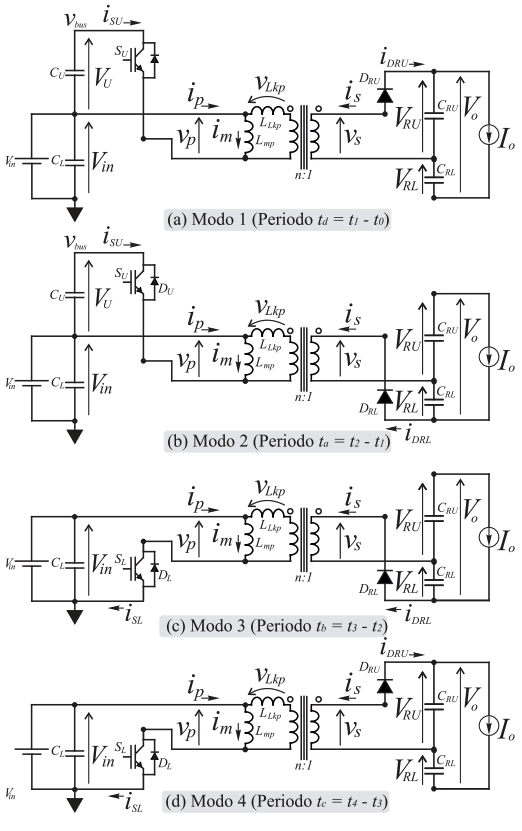
\includegraphics[width=0.7\linewidth]{img/modosOperacion}
	\caption{Modos de operación del convertidor.}
	\label{fig:modosoperacion}
\end{figure}


\subsubsection{Modo 1}

En el instante \( t_0 \), cuando se apaga el interruptor \( S_L \), la corriente \( i_p \) alcanza su valor máximo positivo \( i_p(t_0) \) y pasa instantáneamente a circular por el diodo  \( D_U \) del interruptor \( S_U \). El circuito correspondiente a este intervalo se muestra en la Fig. 3-4(a). En este modo de operación, la tensión aplicada al primario del transformador es \( v_p = -V_U \). La corriente del secundario circula por el diodo \( D_{RU} \), aplicando una tensión \( v_s = V_{RU} \) al secundario del transformador, y una tensión \( v_{LKp} = -(V_U + nV_{RU}) \) sobre la inductancia de dispersión. Así, durante este intervalo, la corriente \( i_m \) decrece con pendiente \( -V_U / L_{mp} \) y la corriente por la inductancia de dispersión decrece con pendiente \( -(V_U + nV_{RU}) / L_{LKp} \). La corriente \( i_p \) por el primario del transformador (suma de la corriente por la inductancia de magnetización y la corriente por la inductancia de dispersión) decrece con pendiente:

\[
-p_3 = -\left( \frac{V_U}{L_p} + n \frac{V_{RU}}{L_{LKp}} \right)
\]

donde \( L_p = L_{LKp} \parallel L_{mp} \). Luego del intervalo \( t_D \) (tiempo muerto), contado a partir de \( t_0 \), se activa el gate del IGBT \( S_U \). El encendido de \( S_U \) se realiza a tensión y corriente cero, pues \( i_p \), que es positiva, circula en ese instante por el diodo en antiparalelo con \( S_U \), evitando pérdidas de conmutación. Este modo finaliza en el instante \( t_1 \), cuando la corriente \( i_p \) iguala a la corriente \( i_m \), momento en el que \( D_{RU} \) se apaga naturalmente cuando su corriente se hace cero.

\subsubsection{Modo 2}

Al inicio de este modo de operación, la corriente que circula por el primario del transformador es igual a la corriente por la inductancia de magnetización, con un valor de \( i_p(t_1) \). Después del instante \( t_1 \), la corriente \( i_p \) se vuelve menor que la corriente de magnetización \( i_m \), haciendo que la corriente del secundario circule por el diodo \( D_{RL} \). . La corriente \( i_{DRL} \) crece desde cero con una pendiente limitada, evitando pérdidas durante el encendido del diodo \( D_{RL} \). La tensión aplicada sobre la inductancia de magnetización sigue siendo \( v_p = -V_U \), mientras que la tensión en el secundario del transformador es \( v_s = -V_{RL} \). Por lo tanto, la corriente \( i_m \) decrece con pendiente \( -\frac{V_U}{L_{mp}} \) y la corriente por la inductancia de dispersión decrece con pendiente \( -\frac{V_U - nV_{RL}}{L_{LKp}} \). La corriente \( i_p \) decrece con pendiente:

\[
-p_4 = -\left( \frac{V_U}{L_p} + n \frac{V_{RL}}{L_{LKp}} \right)
\]

donde \( L_p = L_{LKp} \parallel L_{mp} \). El Modo 2 finaliza en \( t_2 = dT \), cuando se apaga el IGBT \( S_U \).

\subsubsection{Modo 3}

Cuando se apaga el IGBT \( S_U \), la corriente \( i_p \) alcanza su máximo negativo \( i_p(t_2) \) y pasa instantáneamente a circular por \( D_L \) del IGBT \( S_L \). El diodo \( D_{RL} \) del rectificador permanece en conducción, y su corriente comienza a decrecer. La tensión sobre la inductancia de magnetización del transformador pasa a ser \( v_p = V_{in} \), mientras que la tensión en el secundario sigue siendo \( v_s = -V_{RL} \). La corriente \( i_m \) crece con pendiente \( \frac{V_{in}}{L_{mp}} \), y la corriente por la inductancia de dispersión crece con pendiente \( \frac{V_{in} + nV_{RL}}{L_{LKp}} \). La corriente por el primario crece con la pendiente:

\[
p_1 = \left( \frac{V_{in}}{L_p} + n \frac{V_{RL}}{L_{LKp}} \right)
\]

donde \( L_p = L_{LKp} \parallel L_{mp} \). Para asegurar el encendido a tensión y corriente cero de \( S_L \), la activación de este IGBT debe hacerse antes de que la corriente \( i_p \) cambie de signo. Esta es una condición de diseño para el correcto funcionamiento del convertidor, asegurando que en el instante de activación la corriente esté circulando por el diodo de recuperación inversa \( D_L \). Este modo finaliza en el instante \( t_3 \) cuando la corriente \( i_p \) iguala a la corriente \( i_m \), momento en el que el diodo \( D_{RL} \) del rectificador se apaga naturalmente al alcanzar su corriente cero.

\subsubsection{Modo 4}

Durante este intervalo, la corriente \( i_p \) que entra al primario del transformador supera a la corriente de magnetización \( i_m \), lo que lleva al encendido del diodo \( D_{RU} \). Este modo de operación coincide con el circuito ilustrado en la Figura 3-4(d). La tensión en el primario del transformador permanece como \( v_p = V_{in} \), mientras que la tensión en el secundario se convierte en \( v_s = V_{RU} \). La corriente \( i_m \) aumenta con una pendiente de \( \frac{V_{in}}{L_{mp}} \), y la corriente a través de la inductancia de dispersión aumenta con una pendiente de \( \frac{V_{in} - nV_{RU}}{L_{LKp}} \). La corriente \( i_p \) también aumenta con una pendiente dada por:

\[
p_2 = \left( \frac{V_{in}}{L_p} - n \frac{V_{RU}}{L_{LKp}} \right)
\]

donde \( L_p = L_{LKp} \parallel L_{mp} \) (3-6). Este modo de operación concluye en \( t_4 = T_s \), momento en que se apaga el IGBT \( S_L \) y se reinicia al Modo 1.

\subsection{Estado estacionario}

Para caracterizar a un convertidor como el trabajado en este informe, se desea conocer su ganancia en tensión $V_o/V_{in}$. Se sabe que este circuito no tiene un comportamiento lineal, por lo que no se puede hallar una ecuación cerrada que exprese la ganancia. Para ello, se toma como referencia del material bibliográfico, un estudio realizado, que obtiene de manera analítica un conjunto de cuatro ecuaciones no lineales con cuatro incógnitas, que definen el comportamiento del convertidor en estado estacionario y permiten encontrar su ganancia de tensión para cualquier punto de operación. Para no depender de la relación de transformación, se trata con las tensiones intervinientes referidas al primario del transformador. 

Se tiene la siguiente \hyperref[fig:corrienteestacionario]{característica de la forma de onda de corriente para estado estacionario}.

\begin{figure}
	\centering
	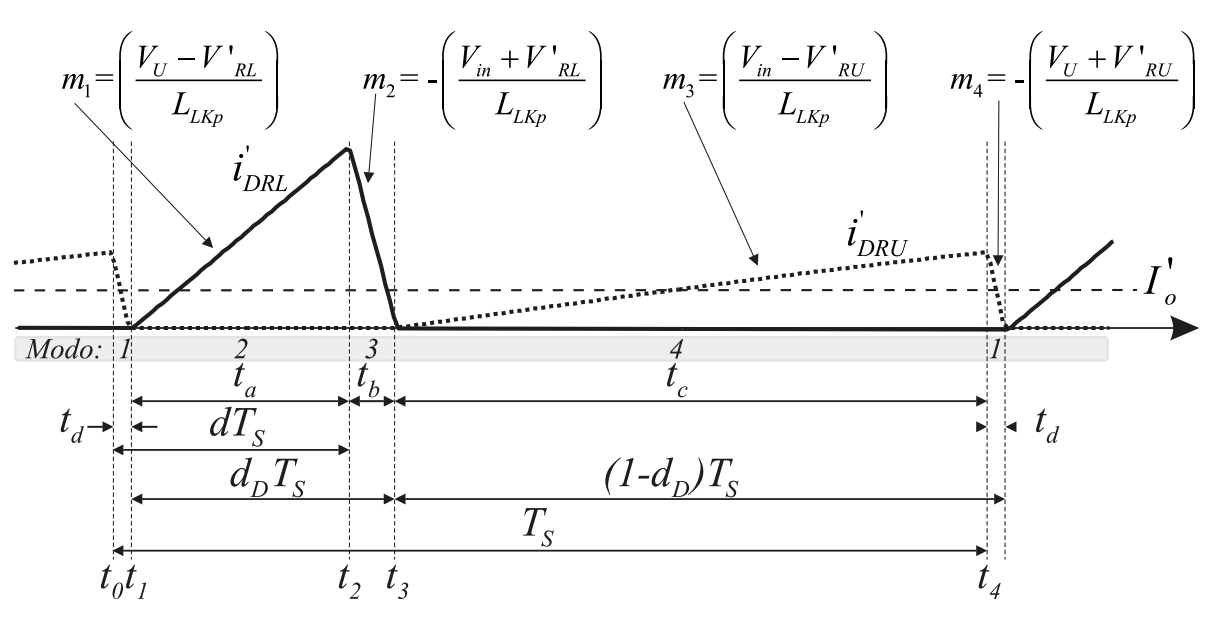
\includegraphics[width=0.7\linewidth]{img/corrienteEstacionario}
	\caption{}
	\label{fig:corrienteestacionario}
\end{figure}

En donde las pendientes están dadas por:

$$
\begin{cases}
	m_1 = \frac{V_U - V_0}{R_L L_{LKp}} \\
	m_2 = -\frac{V_{in} + V_0}{R_L L_{LKp}} \\
	m_3 = \frac{V_{in} - V_0}{R_U L_{LKp}} \\
	m_4 = -\frac{V_U + V_0}{R_U L_{LKp}}
\end{cases}
$$

Finalmente, las cuatro incógnitas son:

\begin{itemize}
	\item $V_{RU}'$
	\item $V_{bus}$
	\item $t_b$
	\item $t_d$
\end{itemize}

Siendo posible resolver de forma numérica ecuaciones para obtener valores para cada punto específico de operación dado por:

\begin{itemize}
	\item $V_{in}$
	\item $I_o'$
	\item $V_o'$
\end{itemize}

Y a partir de esto obtener la relación $V_o'/V_{bus}$ deseada. Entonces, el sistema de cuatro ecuaciones que modelan el comportamiento del convertidor es:

$$
\begin{cases}
	[V_{bus(pu)}-V_{in(pu)}-(V'_{o(pu)}-V'_{RU(pu)})]\frac{V'_{RU(pu)}}{V'_{o(pu)}}T_{s(pu)}=V_{bus(pu)}t_{b(pu)} \\
	(V_{in(pu)}-V'_{RU(pu)})\left(\frac{V'_{o(pu)}-V'_{RU(pu)}}{V'_{o(pu)}}\right)T_{s(pu)}=V_{bus(pu)}t_{b(pu)} \\
	I'_{o(pu)} = \frac{V'_{RU(pu)}}{2V'_{o(pu)}} \left(\frac{V_{in(pu)}+V'_{o(pu)}-V'_{RU(pu)}}{L_{LKp(pu)}}\right) 2\pi t_{b(pu)} \\
	I'_{o(pu)} = \frac{V'_{o(pu)}-V'_{RU(pu)}}{2V'_{o(pu)}} \left(\frac{V_{bus(pu)}-V_{in(pu)}+V_{RU(pu)}}{L_{LKp(pu)}}\right)2\pi t_{d(pu)}\
\end{cases}
$$

Se logran las siguientes curvas de regulación para las ecuaciones anteriores.

\begin{figure}
	\centering
	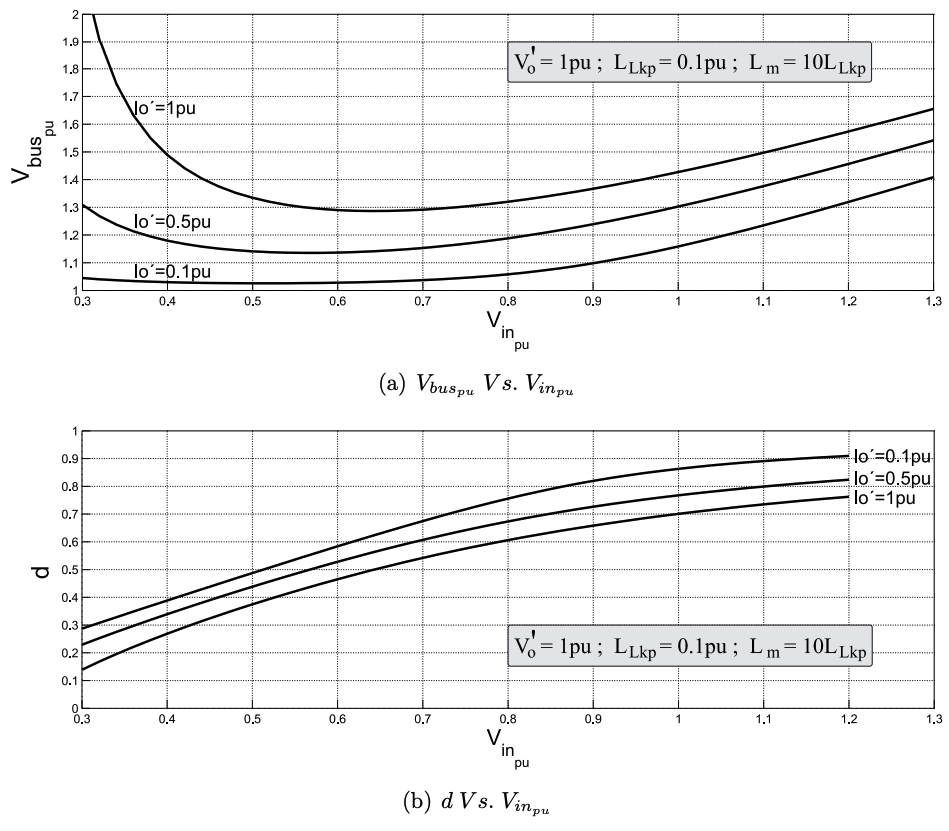
\includegraphics[width=0.9\linewidth]{img/eqV}
	\caption{(a) $d \ vs. \ V_{in(pu)}$ y (b) $V_{bus(pu)} \ vs. \ V_{in(pu)}$; para $V'_{o(pu)}=1$ parametrizada en $I'_{o(pu)}$.}
	\label{fig:eqv}
\end{figure}

\begin{figure}
	\centering
	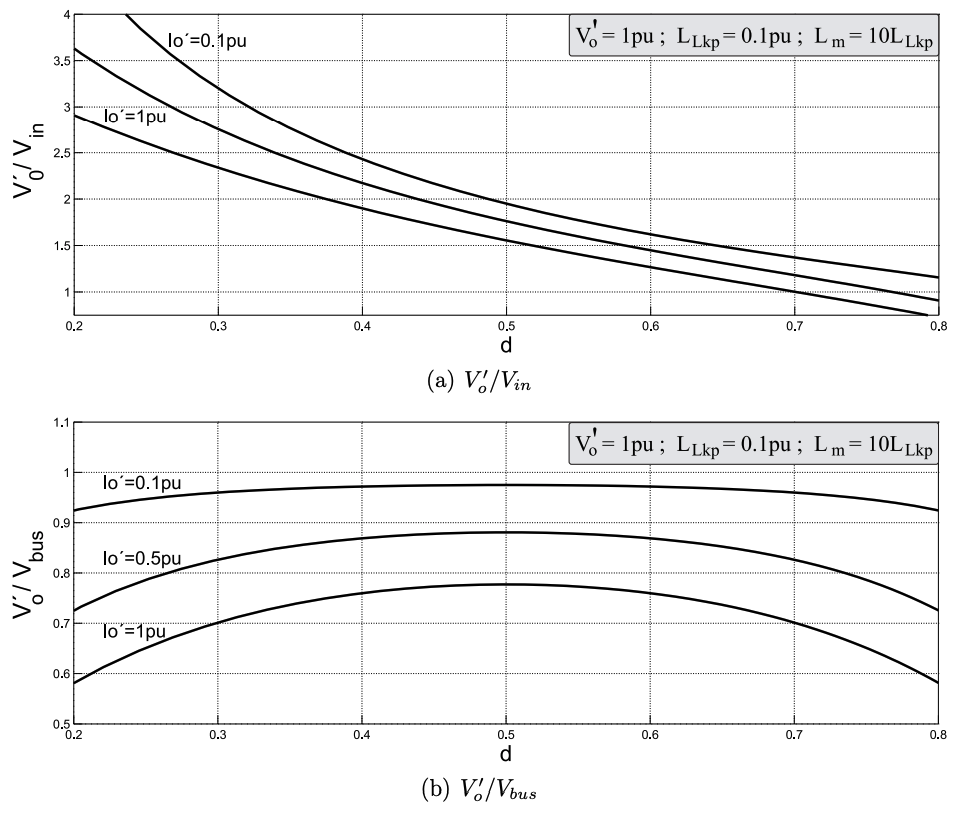
\includegraphics[width=0.9\linewidth]{img/eqI}
	\caption{Ganancias del convertidor en función del ciclo de trabajo $d$ y de la corriente de salida $I'_{o(pu)}$.}
	\label{fig:eqi}
\end{figure}


\subsection{Conmutación suave}

También llamada ZVS (Zero Voltage Switching), se puede lograr bajo cierta condiciones y con un determinado rango de tensión de entrada y corriente de salida. El rango de conmutación suave está definido por la relación entre la inductancia de magnetización y la inductancia de dispersion del transformador $L_{mp}/L_{LKp}$, por el valor de los capacitores de snubber $C_r$ y el tiempo muerto $t_D$ entre el apagado de un IGBT y el encendido del otro.

\subsubsection{Encendido a tensión cero de $S_U$}

Esto es fácil de lograr, cuando se apaga $S_L$, $i_P$ pasa a circular por el diodo $D_U$, haciendo que la tensión se vaya a cero. En este momento $i_P$ está en su máximo valor positivo, por lo que se tiene un tiempo considerable para encender $S_U$ antes de que la corriente cambie de signo y despolarice el diodo $D_U$.

\subsubsection{Encendido a tensión cero de $S_L$}

Este encendido es más crítico que el anterior. En el instante $t_2$, cuando se apaga $S_U$, la corriente $i_P$ alcanza su mínimo y pasa a circular por el diodo $D_L$. La magnitud mínima $i_P(t_2)$ puede ser pequeña y a partir de ese momento la corriente por el primario del transforamdor comienza a crecer con una pendiente elevada, $p_1$. De esta forma, el tiempo muerto $t_D$ máximo a usar es reducido.

\begin{figure}
	\centering
	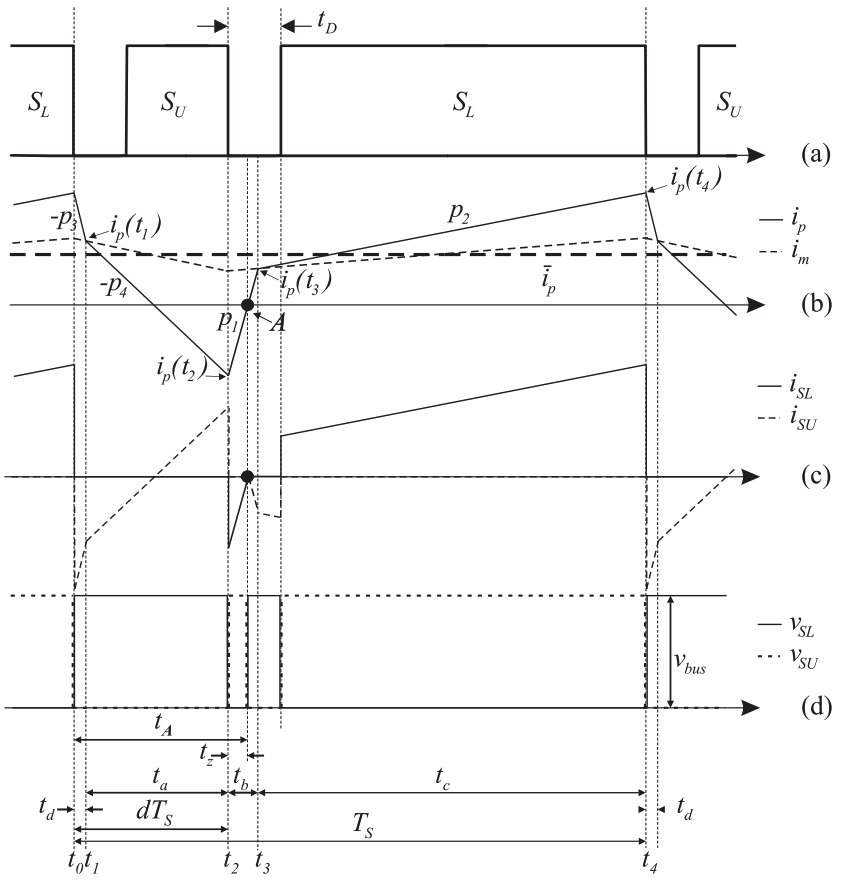
\includegraphics[width=0.7\linewidth]{img/suave1}
	\caption{Curvas para \( t_D > t_z \): (a) Señales de encendido $S_U$ y $S_L$. (b) \( i_p \), \( \bar{i}_p \) e \( i_m \). (c) \( i_{SL} \) e \( i_{SU} \). (d) \( v_{SL} \) y \( v_{SU} \).}
	\label{fig:suave1}
\end{figure}

\subsubsection{Tiempo muerto $t_D$}

Luego del apagado de la llave $S_U$, para asegurar que la llave $S_L$ encienda a tensión cero, su activación debe realizarse antes de que $i_P$ cambie de negativa a positiva. Si se define $t_A$ como el tiempo contado desde $t_0$, hasta el instante en que la corriente cruza por cero en el punto A, y se define $t_z=(t_A-t_2)$ como el tiempo que tarda la corriente $i_P$ en cruzar por cero luego del momento $t_2$ en que se apagó $S_U$, para que la llave $S_L$ encienda a tensión cero, debe ser $t_D<t_z$.

\begin{figure}
	\centering
	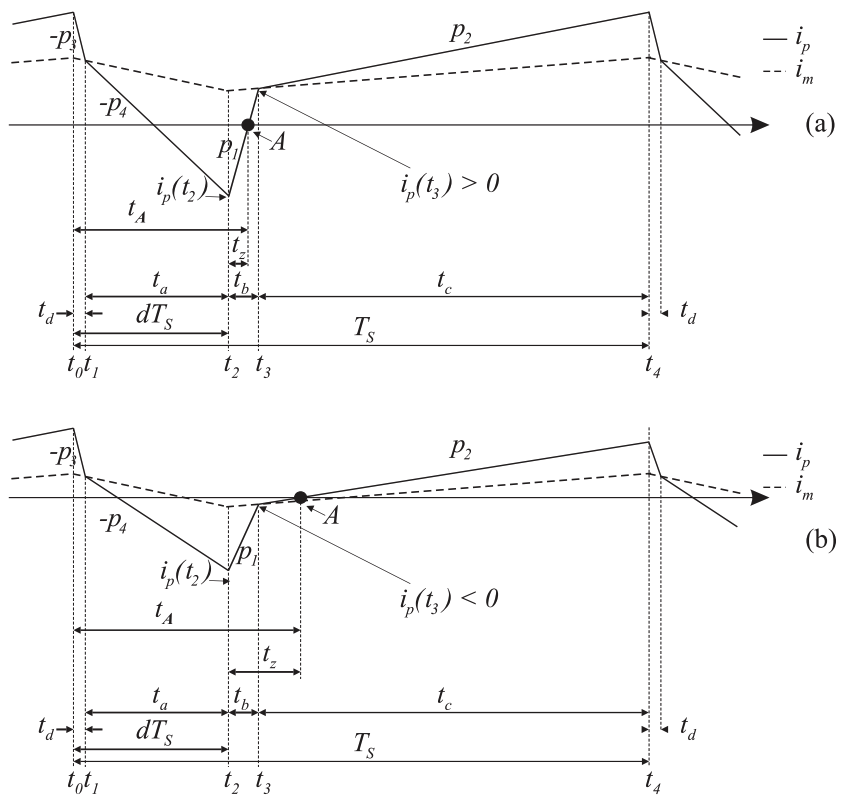
\includegraphics[width=0.8\linewidth]{img/tD}
	\caption{Forma de onda de las corrientes $i_P$ e $i_m$ para: (a) $i_m(t_3)>0$ y (b) $i_m(t_3)<0$.}
	\label{fig:td}
\end{figure}

Resulta necesario limitar el valor mínimo de la relación $L_{mp}/L_{LKp}$, además, al aumentar esta relación disminuye $t_{z(min)}$. Esto no es conveniente porque limita el tiempo muerto $t_D$, que es el tiempo que tienen las llaves en el apagado para llevar a cero las corrientes y realizar la carga o descarga de los capacitores de snubber. Por eso se define como relación de compromiso $L_{mp}/L_{LKp}=10$. Siendo que, para que el convertidor opere en conmutación suave en todo el rango $0.42<V_{in(pu)} < 0.9$, debe utilizarse un tiempo muerto $t_D\leq 0.48 \ \mu s$.

\subsubsection{Efecto de los capacitores de snubber $C_r$}

Los capacitores de snubber tienen la función de retardar el aumento de la tensión sobre las llaves $S_L$ y $S_U$ durante su apagado. Esto es esencial porque las llaves no pueden apagarse instantáneamente, sino que requieren un tiempo finito, conocido como tiempo de caída. Durante este período, es crucial retrasar el aumento de la tensión para minimizar las pérdidas. Aunque es deseable que los capacitores de snubber sean grandes para maximizar este retardo, se debe tener cuidado. Un exceso de tamaño podría retrasar también la caída de tensión en la llave próxima a encenderse, lo que resultaría en pérdidas adicionales durante su encendido.

\begin{figure}
	\centering
	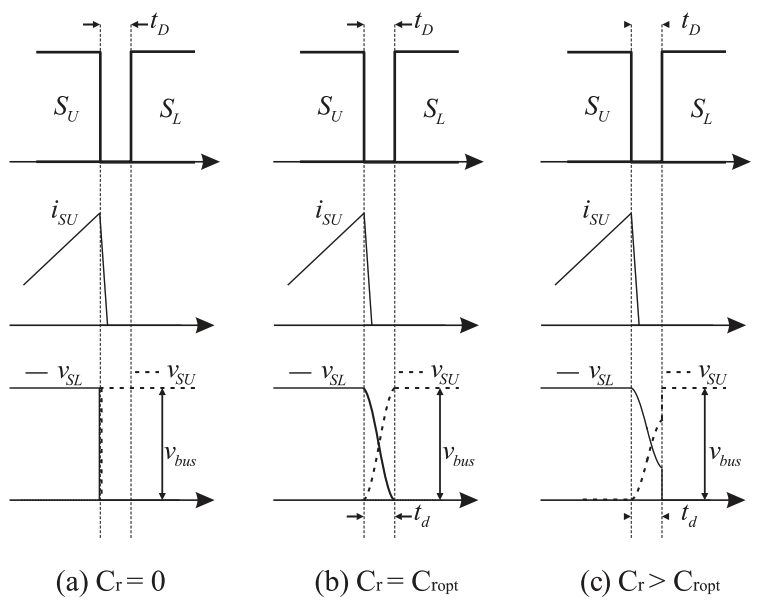
\includegraphics[width=0.6\linewidth]{img/capSnubber}
	\caption{Señales de encendido de $S_L$ y $S_U$, corriente $i_{SU}$ y tensiones $v_{SU}$ para distintos casos de valores de capacitancia de snubber.}
	\label{fig:capsnubber}
\end{figure}

Para cada punto de operación del convertidor debe existir un valor óptimo de los capacitores de snubber $C_{ropt}$, que haga que la tensión sobre la llave próxima a encenderse llegue a cero justo en el instante de encendido.

\subsubsection{Diseño de los capacitores de snubber $C_r$}

\begin{figure}
	\centering
	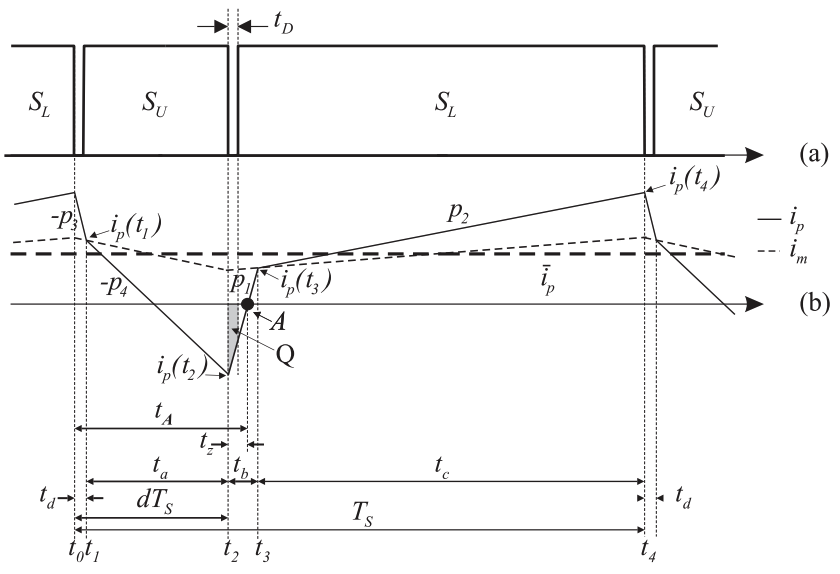
\includegraphics[width=0.6\linewidth]{img/energiaQ}
	\caption{Energía $Q$ utilizada para el dimensionamiento de los capcaitores de snubber.}
	\label{fig:energiaq}
\end{figure}

Para calcular el valor máximo que pueden tener los capacitores de snubber $C_r$, a fin de que la tensión haya llegado a cero antes de que se encuenda la llave $S_L$ en todo el rango de operación del convertidor, se calcula el área de la corriente $i_P$ durante el intervalo sombreado en la \hyperref[fig:energiaq]{figura 10}. Se define de esa manera $C_{r0}=Q/2V_{bus}$, $C_{r(pu)}=2\pi R_B C_{r0}/T_B$, aproximando de esa forma un valor $C_{r(pu)} \approx 0.02$ que asegura la conmutación suave para el rango de tensión $0.42 < V_{in(pu)} < 0.9$.


\clearpage


\section{Diseño del convertidor}

\subsection{Características deseadas}

Se parte del hecho de que cada panel solar tiene una potencia de aproximadamente $5 \ kWp$. Luego, con el fin de no sobredimensionar componentes tales como el transformador y cada componente del convertidor, se decide por utilizar 4 convertidores DC-DC en paralelo, de forma que aporten cada uno aproximadamente $1/4$ de la corriente de salida solicitada por medio de los requisitos de diseño. 

Se define como máxima tensión de entrada $288 \ V$, la frecuencia de conmutación será de $f_s=50 \ kHz$. El diseño de cada convertidor será de $4 \ kW$Se definen además:

\begin{itemize}
	\item $V'_{oB}=n \ 400 \ V$
	\item $I'_{oB}= \frac{P_n}{nV_o}=\frac{10}{n} \ A$
\end{itemize}

\subsection{Definición de la relación de vueltas del transformador y el rango de tensión de entrada}

Para trabajar en conmutación suave, es conveniente trabajar con:

$$
0.42 < V_{in(pu)} < 0.9
$$

Por lo que se limita $V_{in(pu)} < 0.9$. Ahora, si se reemplaza, se tiene:

$$
n>\frac{V_{in(max)}}{0.9V_{oB}}
$$


Se decide por utilizar como tensión de alimentación $144 \ V$, equivalente a 3 paneles solares en serie. De esa forma, despreciando la caída de tensión en los diodos a la salida, así como la tensión de saturación de los IGBT de la entrada, se obtiene:

$$
n=\frac{400 \ V}{144 \ V} \approx 2.78
$$

Ahora, para contemplar las caídas de tensión de los componentes reales, se utilizará un margen de $5 \%$, logrando $n=2.91$.

\subsection{Definición de los valores de inductancia de dispersión y magnetización del transformador}

La impedancia base del convertidor a implementar viene dada por:

$$
R_B = \frac{V'_{oB}}{I'_{oB}}=\frac{137.45 \ V}{29.1 \ A}=4.72 \ \Omega
$$

El período de conmutación es $T_B=20 \ \mu s$, por lo que:

$$
L_{mp}=\frac{R_B T_B}{2 \pi}=15.02 \ \mu H
$$

Y finalmente:

$$
L_{LKp} = 0.1 \ L_{mp} = 1.5 \ \mu H
$$

\subsection{Definición de los valores de los capacitores}

Se define un valor alto para el capacitor $C_L=100 \ \mu F$ para poder mitigar el ripple de la tensión de entrada. Y, para el otro capacitor, se tiene $C_U=22 \ \mu F$, suavizando así el ripple de $v_{bus}$ y no volviendo muy lenta la dinámica del sistema. 

Ahora, para obtener el valor de los capacitores de salida, se ajustará el valor por simulación, el valor final se verá reflejado en la explicación del siguiente apartado.


\subsection{Inductor de entrada}

Por efectos de la topología, en este caso no es necesario utilizar un inductor de entrada de valor elevado o si quiera colocarlo, se opta por en este caso utilizar un inductor de $1 \ mH$.


\clearpage


\section{Simulación}

\subsection{Simulación ideal}

Para esta simulación se trabaja con PLECS (Plexim). En donde no es necesario implementar circuitos disparadores para los transistores IGBT. La idea es ilustrar una primera aproximación, para luego con otro simulador obtener una salida real.

\subsubsection{Circuito implementado}

Para una simulación con componentes ideales, se trabaja con el software de simulación PLECS, en su versión 4.8 (corriendo en sistema operativo MacOS). Se parte del siguiente esquemático a implementar. 

\begin{figure}
	\centering
	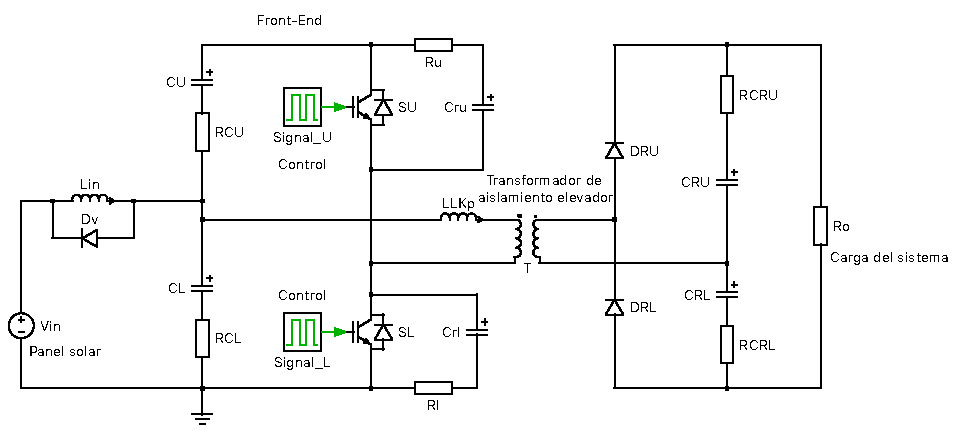
\includegraphics[width=1\linewidth]{../schematic_mod}
	\caption{Circuito esquemático en PLECS.}
	\label{fig:schematic}
\end{figure}

Puede verse algunos cambios en el circuito de alimentación, se mencionan a continuación:

\begin{enumerate}
	\item Se agrega un diodo volante a la inductancia $L_{in}$.
	\item Resistores en serie con los capacitores del sistema.
\end{enumerate}

El diodo volante conectado al inductor $L_{in}$ sirve para proteger el circuito de entrada de una realimentación negativa a la fuente en el caso de que se encuentre operando el circuito sin carga, ya que prácticamente se está teniendo una carga RL.

Los resistores en serie con cada uno de los capacitores se usan a modo de protección contra saltos discretos de los valores de tensión o corriente en los capacitores. Esto es por la forma en que el simulador PLECS interpreta los modelos, en la página web del software recomiendan una resistencia de pequeño valor en serie para poder mitigar estos efectos. Para todos los casos se usan resistores de $1 \ m\Omega$.


\subsubsection{Ajuste de capacitores}

Se realiza un barrido por sobre los capacitores de salida, colocando a ambos del mismo valor. En este barrido se busca medir el ripple por sobre la forma de onda de la tensión. Se toma como referencia la disponibilidad de capacitores de la marca Advance Capacitors, en donde se tiene disponibilidad de capacitores en el rango $5 \ \mu F - 1600 \ \mu F$.

\begin{figure}
	\centering
	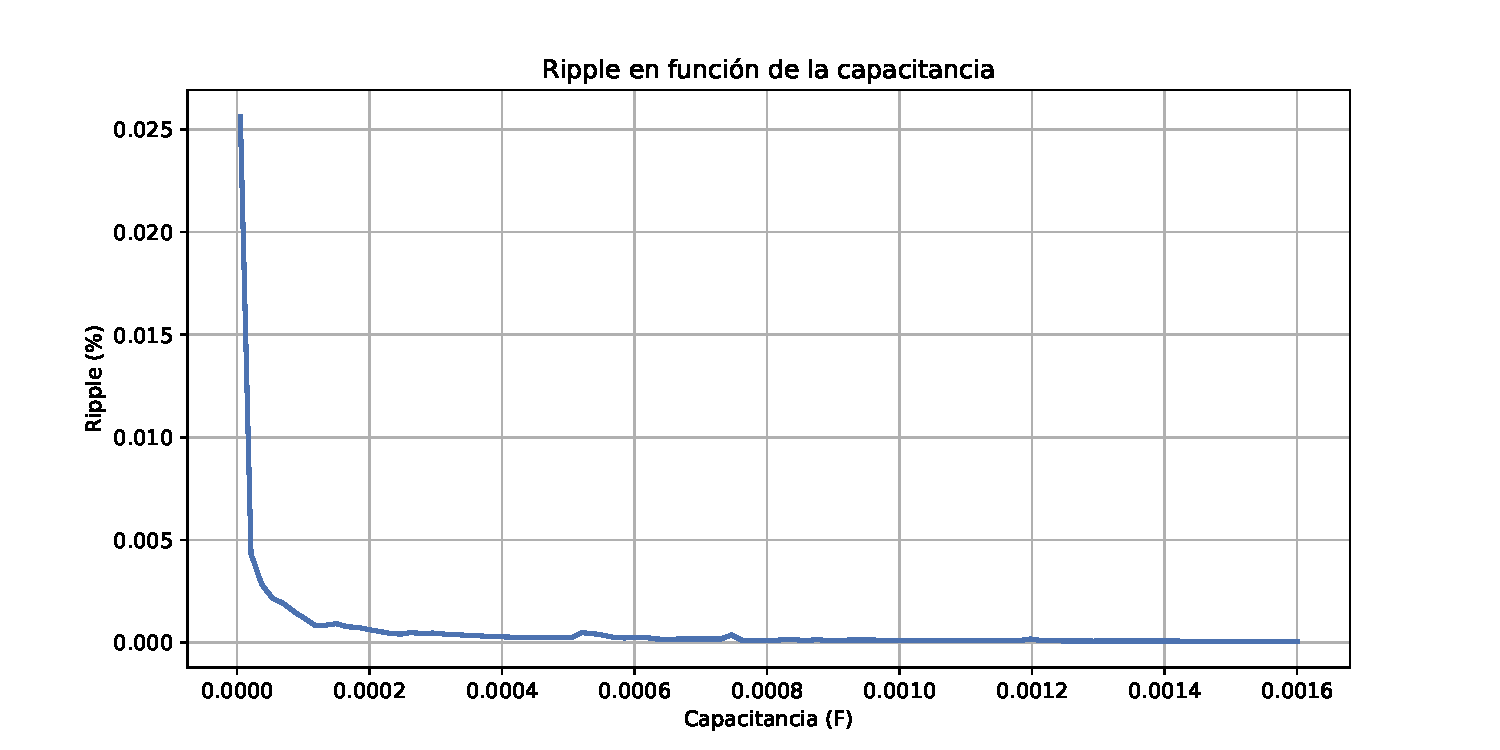
\includegraphics[width=1\linewidth]{../ripple}
	\caption{Variación del ripple con la capacitancia.}
	\label{fig:ripple}
\end{figure}

Puede verse en la figura anterior, cómo claramente el riple disminuye con el aumento de la capacitancia, sin embargo, para valores a partir de $400 \ \mu F$, no disminuye el error prácticamente, por lo que se toma ese como valor final para el diseño, evitando sobredimensionar.

\subsubsection{Señales de disparo de los IGBT}

Se utiliza como referencia, el tiempo muerto de la bilbiografía, que es de $0.48 \ \mu s$, para ello, se parte de un ciclo de trabajo de $d=0.5$, lo que implica que se tiene una señal de disparo para $S_L$ con ese duty cycle y sin delay de fase. Ahora, para el disparo del IGBT inferior, se calcula:

$$d_{SL} = 0.5 - \frac{2\cdot 0.48 \mu s}{20 \ \mu s}=0.452$$

Y, para el delay:

$$t_{SL}=(1-d_{SL})\cdot 20 \ \mu s - 0.48 \ \mu s= 10.48 \ \mu s$$

Se muestran a continuación las formas de onda de las señales de disparo de cada uno de los IGBT. 

\begin{figure}
	\centering
	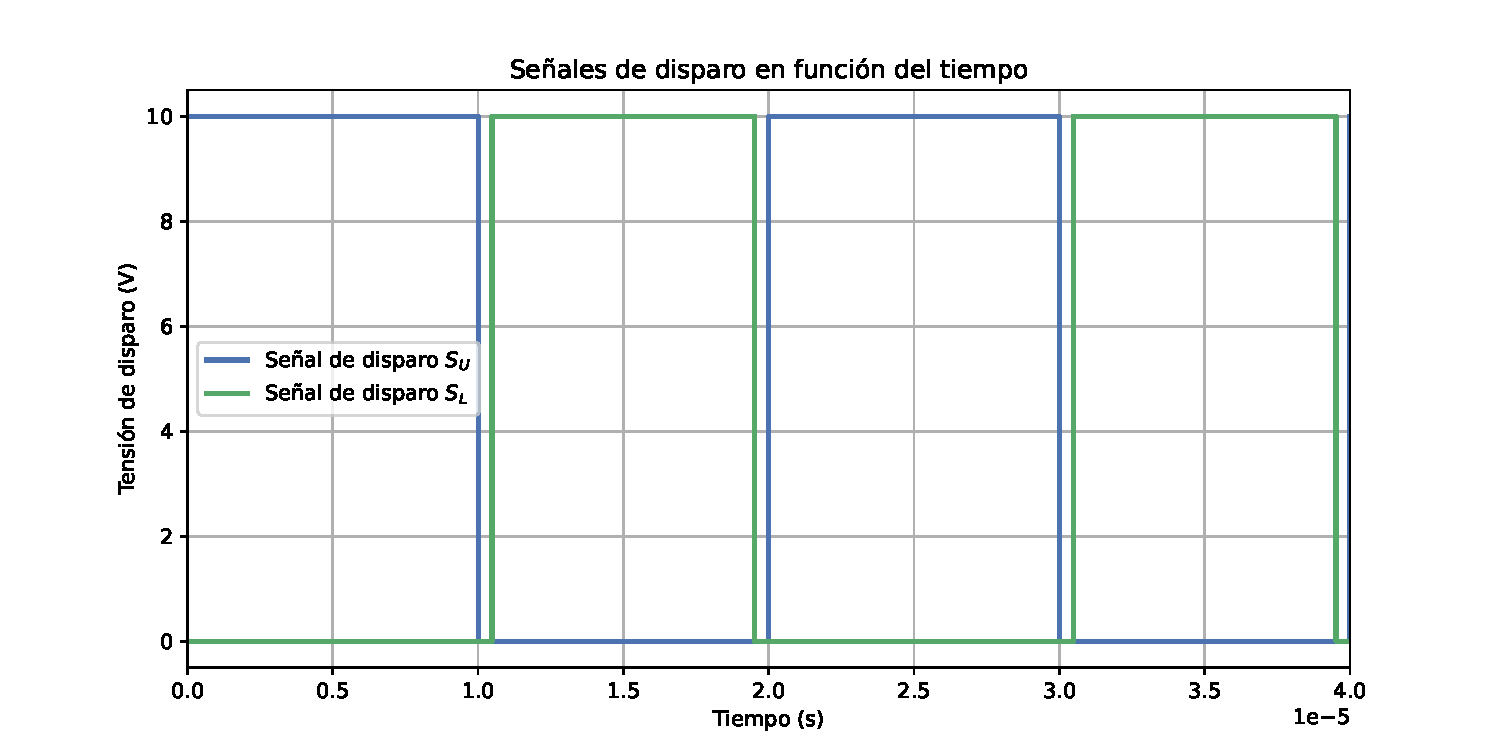
\includegraphics[width=1\linewidth]{../disparo}
	\caption{Señales de disparo de los generadores de pulso.}
	\label{fig:disparo}
\end{figure}

Para este caso ideal, la tensión utilizada para disparar a los transistores es de $10 \ V$. Se puede apreciar la diferencia entre los ciclos de trabajo de cada uno de los trenes de pulso, sin embargo son similares.

\subsubsection{Formas de onda en el transformador}

En cuanto al transformador, se tienen las siguientes formas de onda para las tensiones.

\begin{figure}
	\centering
	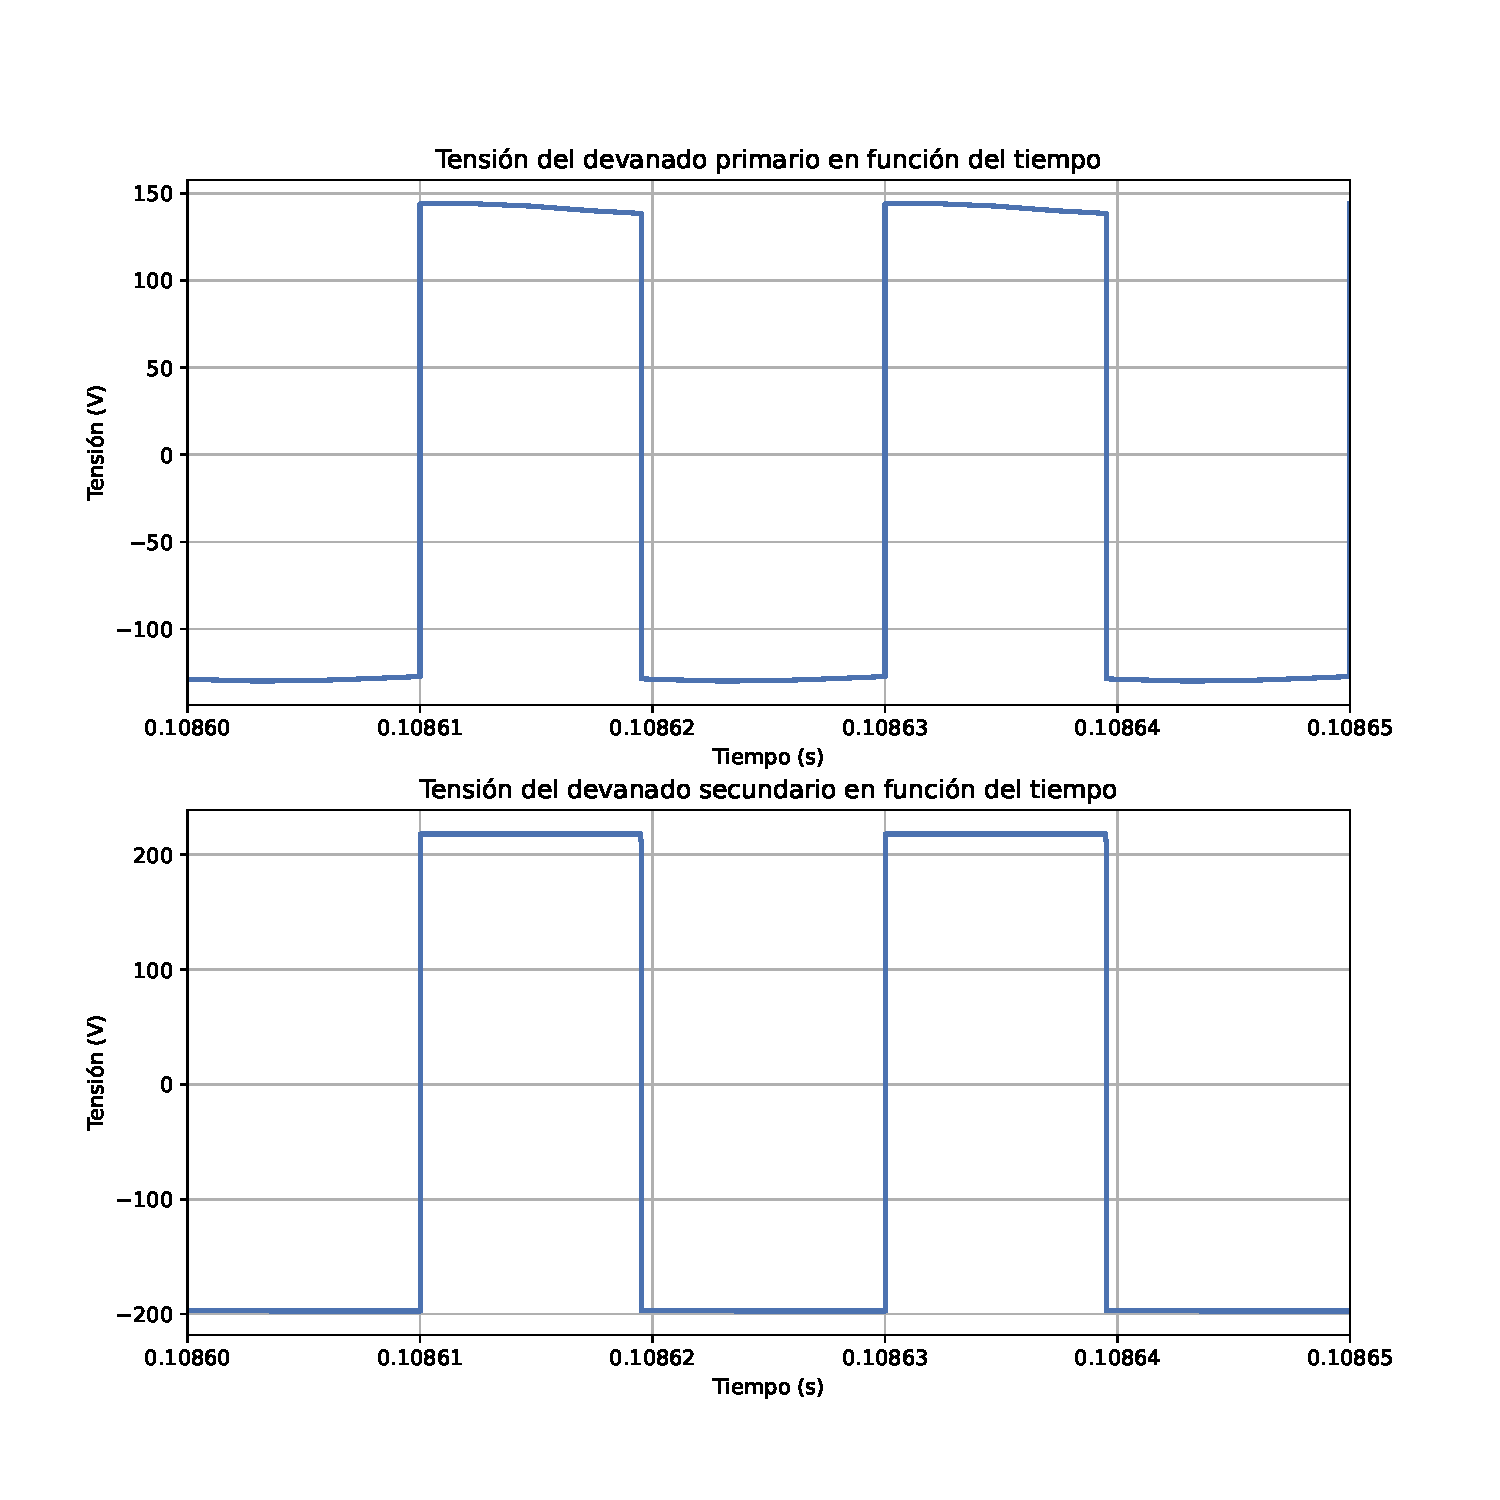
\includegraphics[width=1\linewidth]{../tensiones_transformador}
	\caption{Tensiones en los devanados del transformador.}
	\label{fig:tensionestransformador}
\end{figure}


Ahora, para las corrientes, las formas de onda son las siguientes.

\begin{figure}
	\centering
	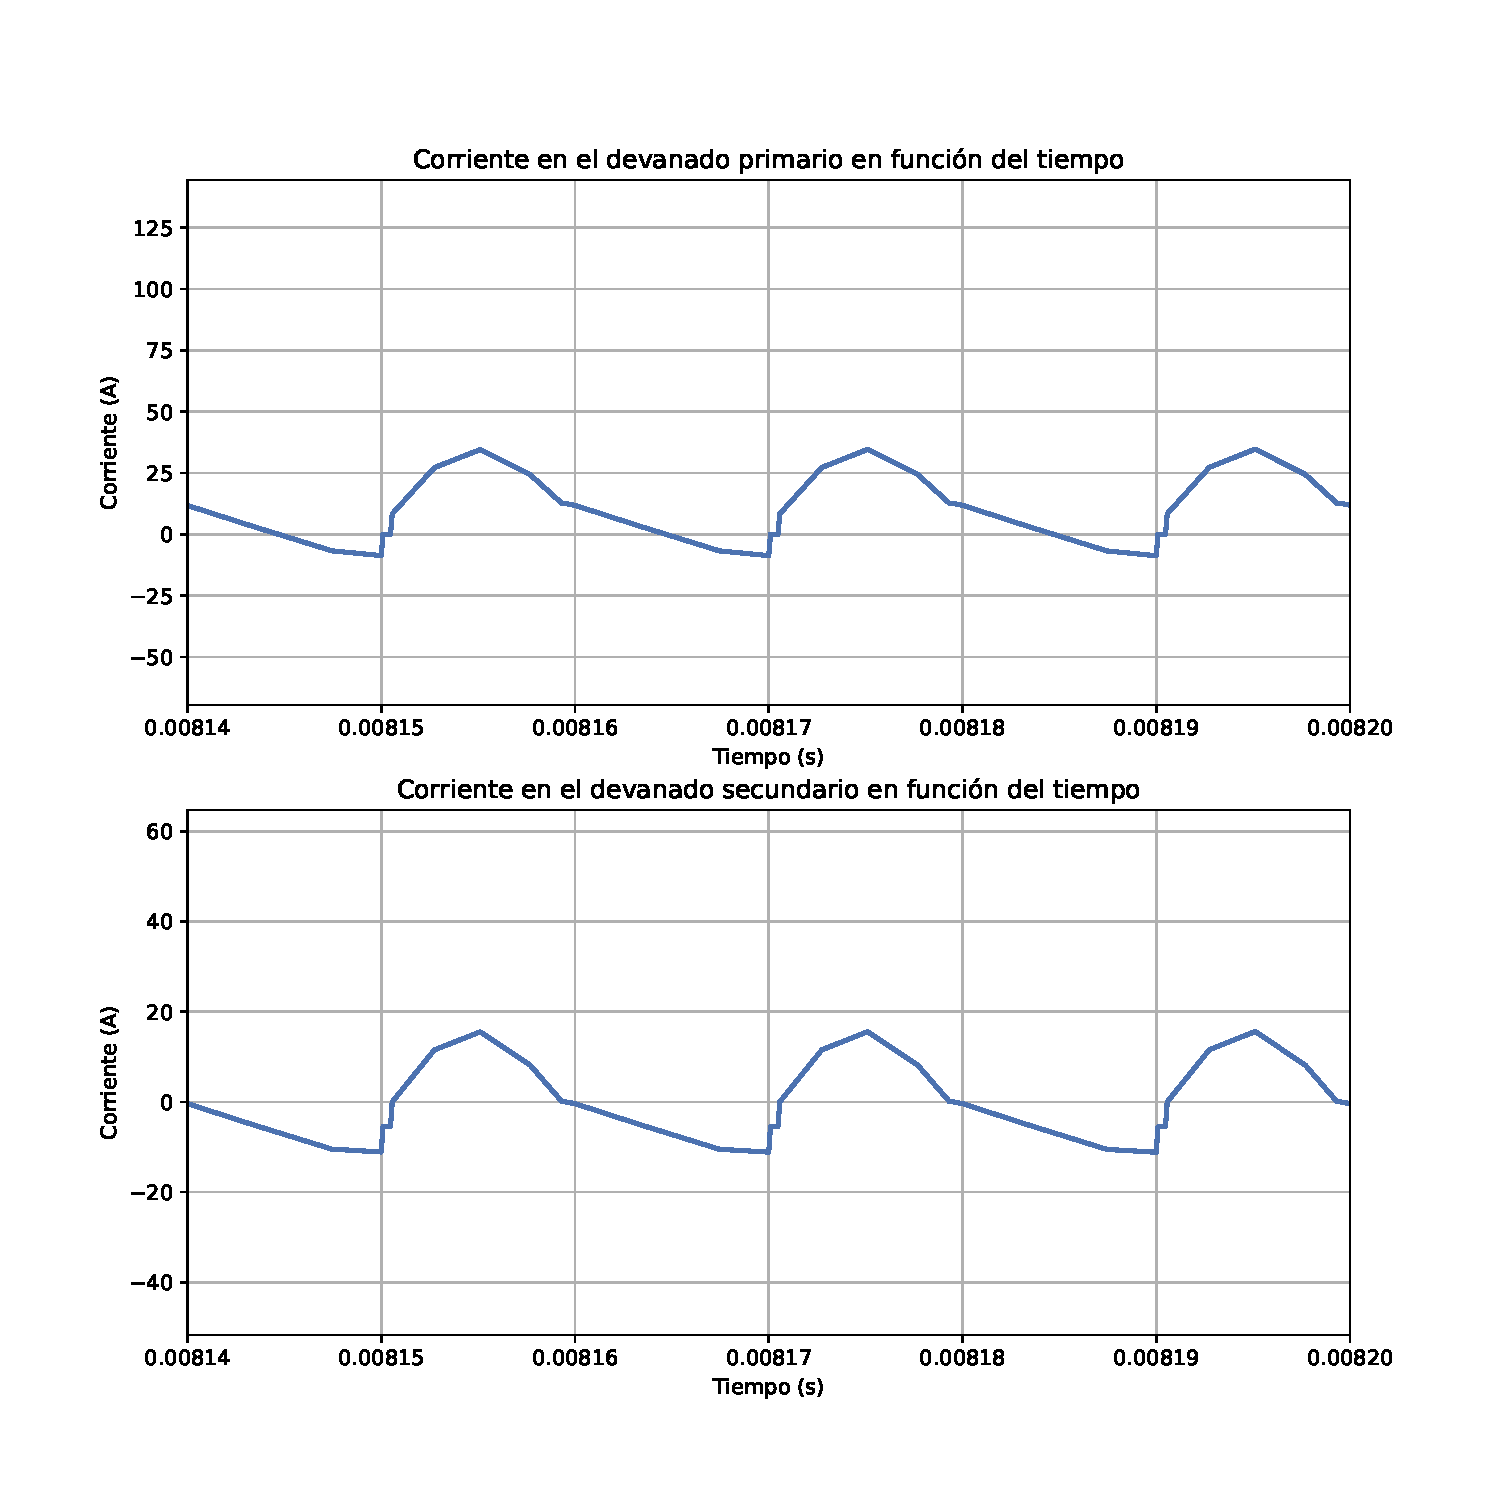
\includegraphics[width=1\linewidth]{../corrientes_transformador}
	\caption{Corrientes en los devanados del transformador.}
	\label{fig:corrientestransformador}
\end{figure}

Pueden apreciarse algunos sobrepicos de corriente, sin embargo el filtro de salida compuesto por el rectificador, así como los capacitores se encargan de no permitir el paso de esos transistorios de la conmutación a la carga.


\subsubsection{Formas de onda de la señal de salida}

Finalmente, las formas de onda más importantes, la salida. En este caso, se toma como referencia una resistencia de $40 \ \Omega$, lo que implica que se está entregando la máxima corriente de diseño para un único convertidor.

\begin{figure}
	\centering
	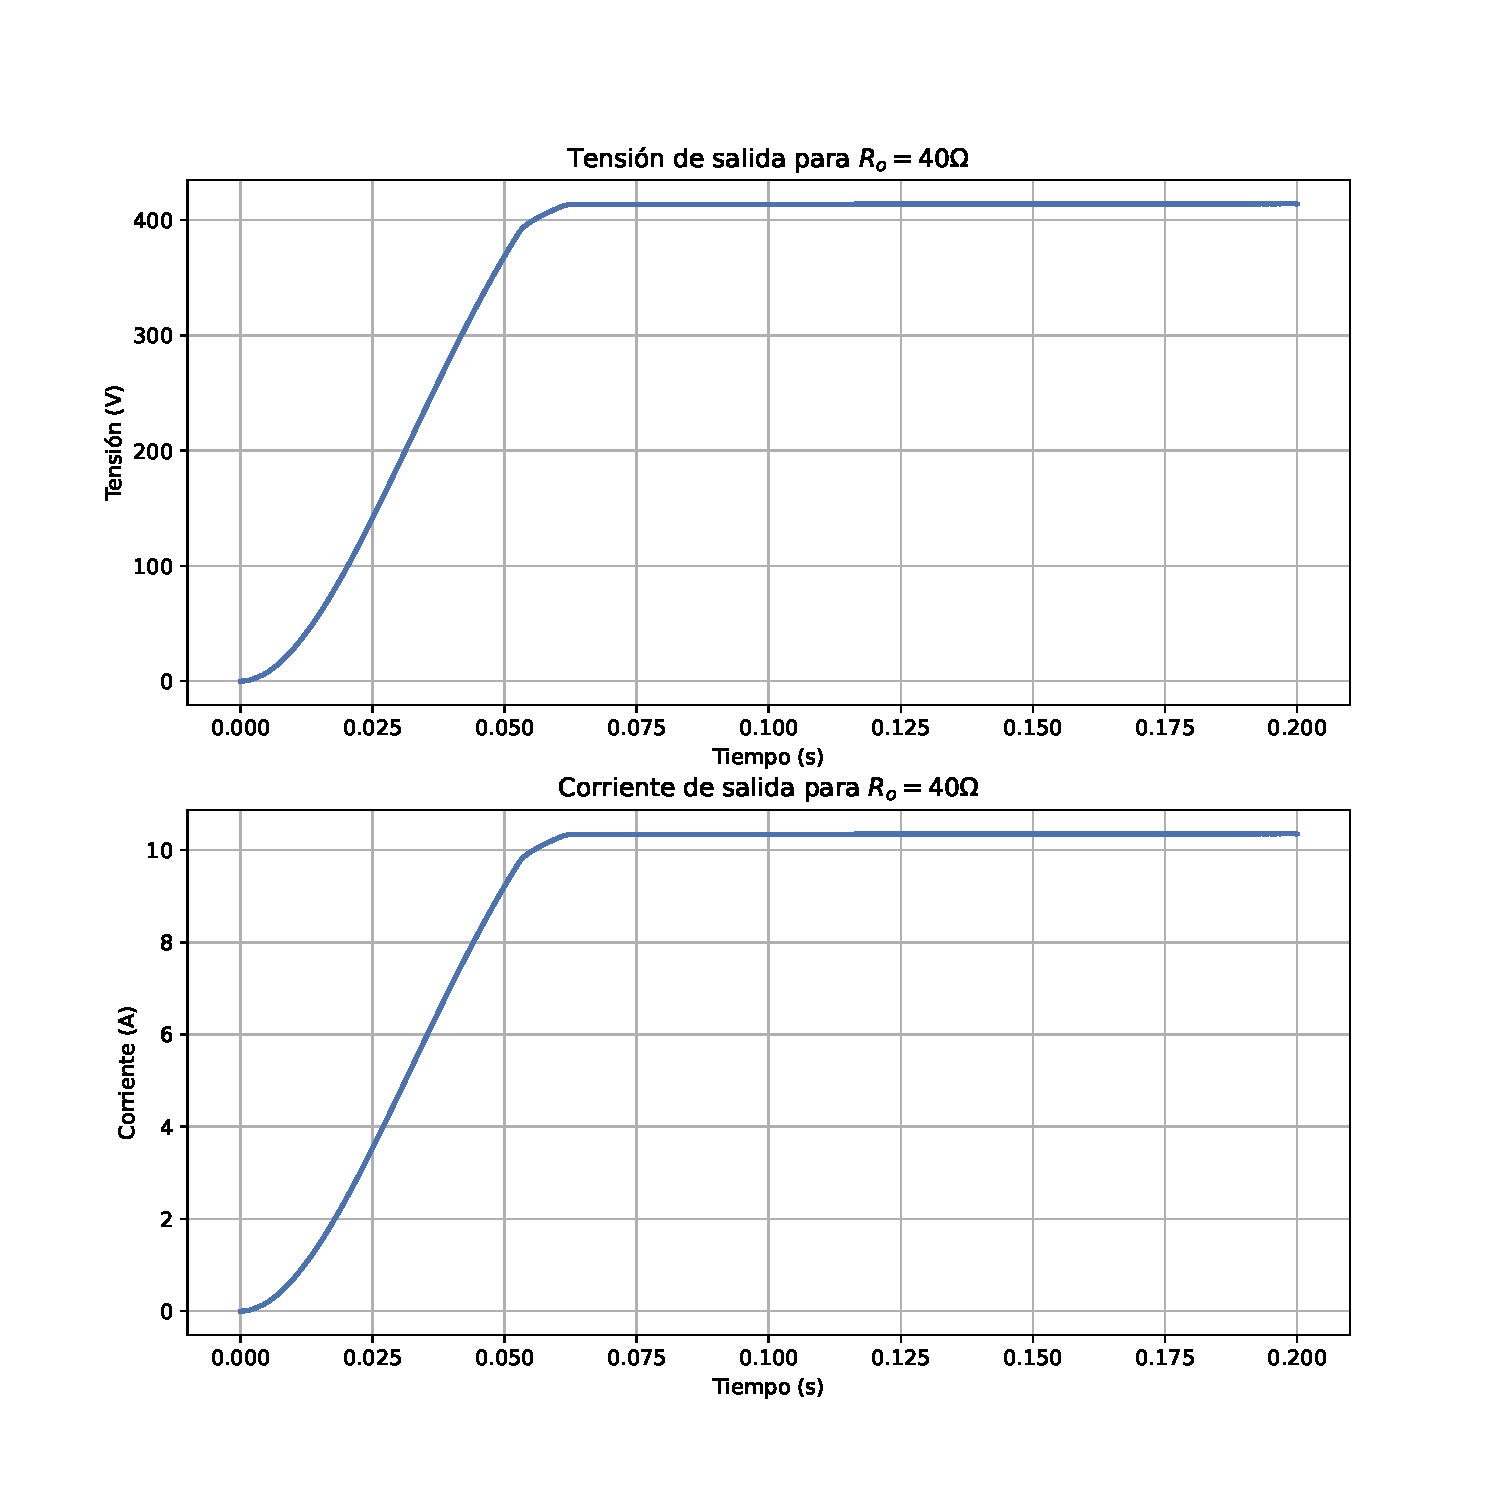
\includegraphics[width=1\linewidth]{../salida_40}
	\caption{Formas de onda a la salida del transformador.}
	\label{fig:salida40}
\end{figure}

Se puede apreciar que no se tienen exactamente los valores medios deseados de $400 \ V$ y $10 \ A$. Esto es por el sobredimensionamiento que se le realizó al transformador para contemplar las pérdidas de los componentes y por el hecho de que la simulación en PLECS no contempla esas no idealidades. Sin embargo, posteriormente en la simulación de un circuito real se podrá apreciar un valor mucho más similar al de diseño.

Ahora, se analiza la regulación del circuito, para ello, se realizará un barrido en la resistencia de salida, de valores entre $40 \ \Omega - 40000 \ \Omega$.

\begin{figure}
	\centering
	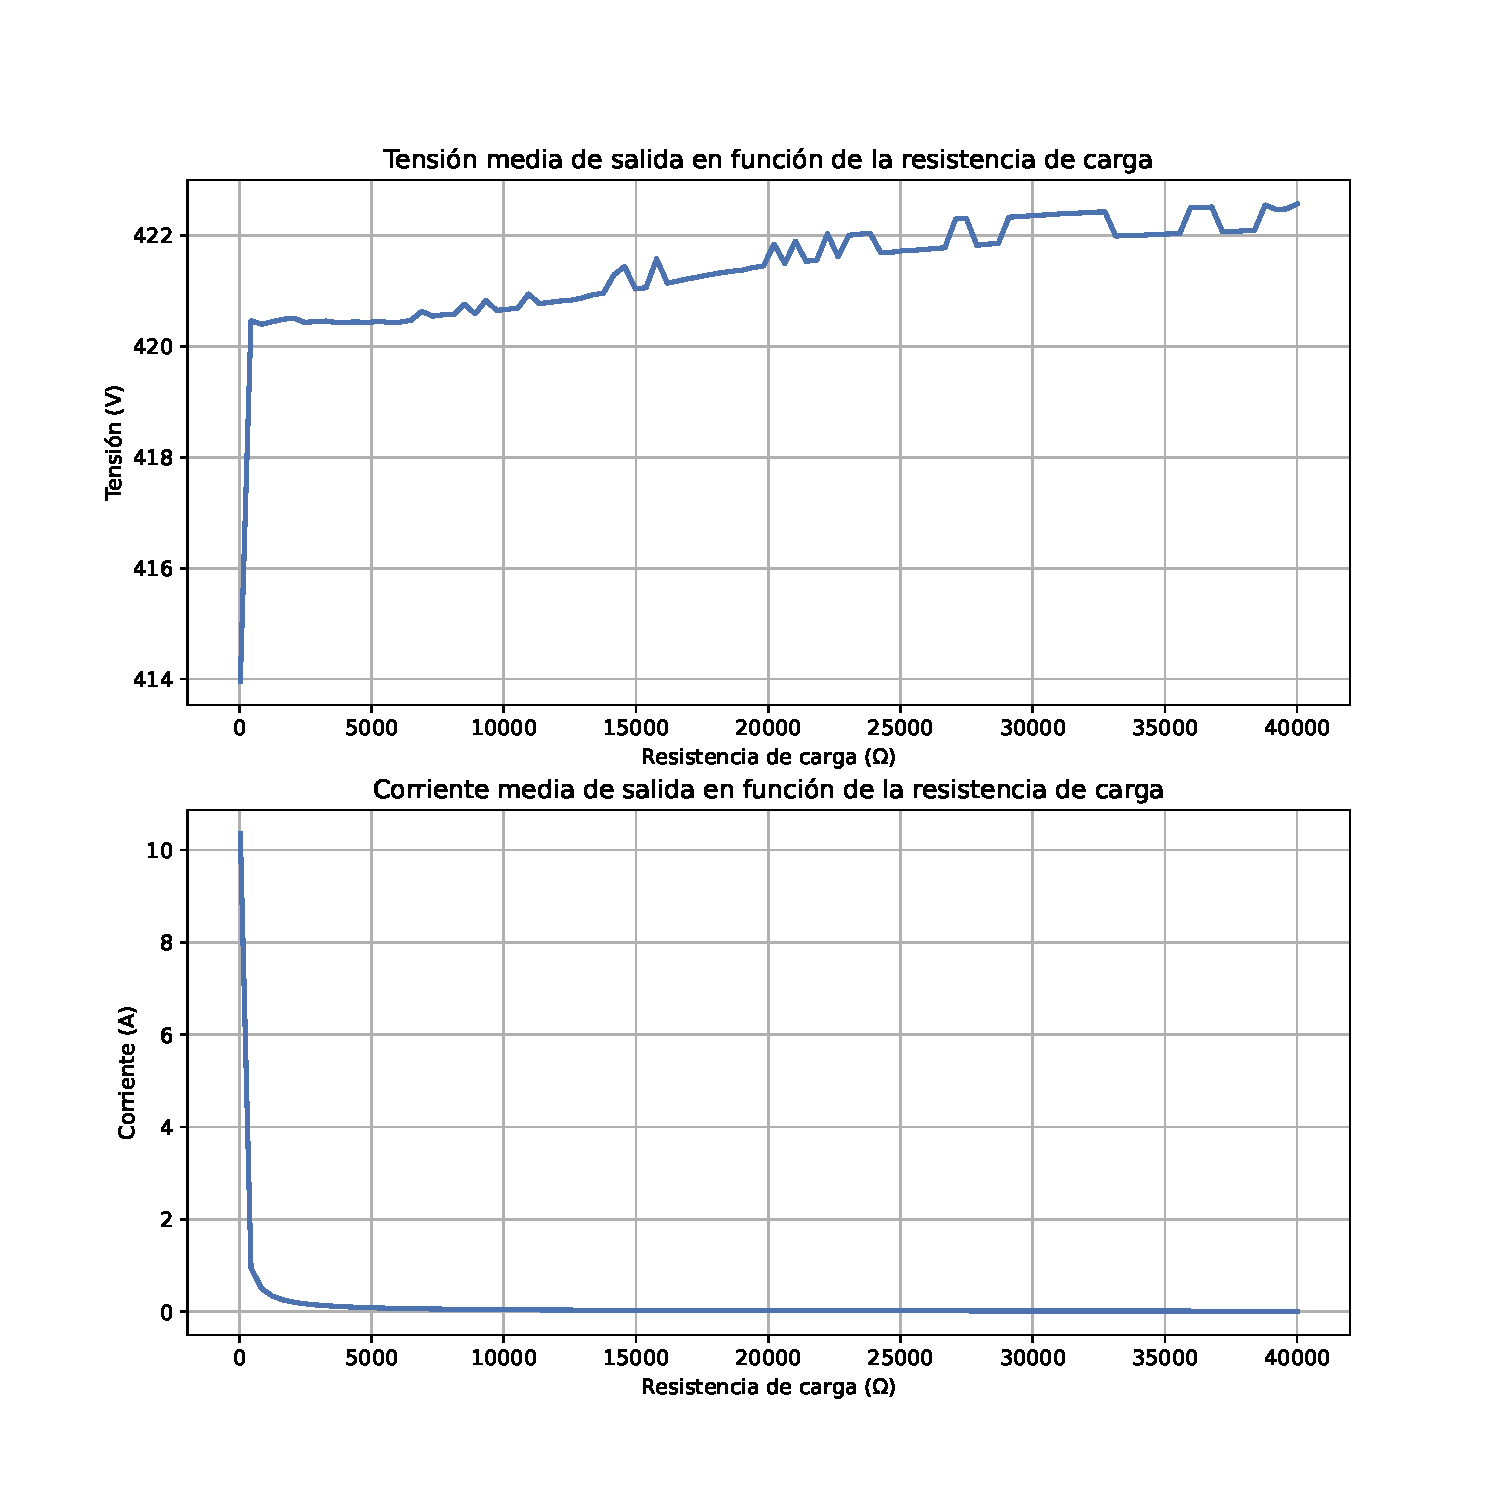
\includegraphics[width=1\linewidth]{../salida_resistencia}
	\caption{Curva de regulación de tensión de salida del convertidor DC-DC diseñado.}
	\label{fig:salidaresistencia}
\end{figure}

Puede verse cómo la salida, que normalmente se establece en $414 \ V$, al aumentar la resistencia se acerca a valores cercanos a $423 \ V$. Se puede ver de esa forma que la regulación individual para cada uno de los convertidores a implementar en paralelo será de aproximadamente $2.17 \%$.












\clearpage

\section{Informes con \LaTeX}

% SUB-SECCIÓN
% Las sub-secciones se inician con \subsection, si se quiere una sub-sección
% sin número se pueden usar las funciones \subsectionanum (nuevo subtítulo sin
% numeración) o la función \subsectionanumnoi para crear el mismo subtítulo sin
% numerar y sin aparecer en el índice
\subsection{Una breve introducción}
	
	Este es un párrafo, puede contener múltiples \quotes{Expresiones} así como fórmulas o referencias\footnote{Las referencias se hacen utilizando la expresión \texttt{\textbackslash label}\{etiqueta\}.} como \eqref{eqn:identidad-imposible} o (\ref{img:anexo-2}). A continuación se muestra un ejemplo de inserción de imágenes (como la Figura \ref{img:testimage}) con el comando \href{https://latex.ppizarror.com/informe.html#hlp-imagen}{\textbackslash insertimage}:

	% Esta instrucción, añadida en la v6.5.5 permite cambiar el título de cada
	% objeto en el índice de cada objeto. Este título es solo válido hasta el
	% primer objeto que lo llame, luego este se restablecerá. Por mientras solo
	% se ofrece compatibilidad para las funciones de imágenes. Los entornos como
	% images o sourcecode aún no tienen compatibilidad
	\setindexcaption{Título de la imagen en el índice.}

	% Para insertar una imagen se puede usar la función \insertimage la cual
	% toma un primer parámetro opcional para definir una etiqueta (dentro de
	% los corchetes), luego toma la dirección de la imagen, sus parámetros
	% (en este caso se definió la escala de 0.12) y una leyenda opcional
	\insertimage[\label{img:testimage}]{ejemplos/test-image.png}{scale=0.12}{Where are you? de \quotes{Internet}.}

	A continuación\footnote{Como se puede observar las funciones \texttt{\textbackslash insert...} añaden un párrafo automáticamente.} se muestra un ejemplo de inserción de ecuaciones simples con el comando \href{https://latex.ppizarror.com/informe.html#hlp-formulae}{\textbackslash insertequation}:

	% Se inserta una ecuación, el primer parámetro entre [] es opcional
	% (permite identificar con una etiqueta para poder referenciarlo después
	% con \ref), seguido de aquello se escribe la ecuación en modo bruto sin signos $
	\insertequation[\label{eqn:identidad-imposible}]{\pow{a}{k}=\pow{b}{k}+\pow{c}{k} \quad \forall k>2}

	% Notar que no se requiere añadir un salto de línea después de insertar una imagen
	Este template \cite{template} ha sido diseñado para que sea completamente compatible con editores \LaTeX\ para escritorio y de manera online\scite{overleaf}. La compilación es realizada siempre usando las últimas versiones de las librerías, además se incluyen los parches oficiales para corregir eventuales \textit{warnings}. \\

	Este es un nuevo párrafo. Para crear uno basta con usar \textbackslash\textbackslash\ en el anterior, lo que fuerza una nueva línea. También se pueden insertar con el comando \texttt{\textbackslash newp} si el compilador de latex arroja una alerta del tipo \textit{Underfull \textbackslash hbox (badness 10000) in paragraph at lines ...}

% SUB-SECCIÓN
\subsection{Añadiendo tablas}

	También puedes usar tablas, ¡Crearlas es muy fácil!. Puedes usar el plugin \href{https://www.ctan.org/tex-archive/support/excel2latex}{Excel2Latex} \cite{excel2latex} de Excel para convertir las tablas a \LaTeX\ o bien utilizar el \quotes{creador de tablas online} \cite{tablesgenerator}.

	% Tabla generada con el plugin Excel2Latex
	\begin{table}[H]
		\centering
		\caption{Ejemplo de tablas.}
		\begin{tabular}{ccc}
			\hline
			\textbf{Columna 1} & \textbf{Columna 2} & \textbf{Columna 3} \bigstrut\\
			\hline
			$\omega$ & $\nu$ & $\delta$ \bigstrut[t]\\
			$\xi$ & $\kappa$ & $\varpi$ \bigstrut[b] \\
			\hline
		\end{tabular}
		\label{tab:tabla-1}
	\end{table}


% ------------------------------------------------------------------------------
% NUEVA SECCIÓN
% ------------------------------------------------------------------------------
\clearpage
\section{Aquí un nuevo tema}

% SUB-SECCIÓN
\subsection{Haciendo informes como un profesional}

	% Se inserta una imagen flotante en la izquierda del documento con
	% \insertimageleft, al igual que las demás funciones, el primer parámetro
	% es opcional, luego viene la ubicación de la imagen, seguido de la escala
	% (un 30% del ancho de página) y por último su leyenda. Para insertar una
	% imagen flotante en la derecha se utiliza \insertimageright usando los
	% mismos parámetros
	\insertimageleft[\label{img:imagen-izquierda}]{ejemplos/test-image-wrap}{0.3}{Apolo flotando a la izquierda.}

	~ \lipsum[1] \\

	% Párrafos de ejemplo
	\lipsum[115]

	% Agrega una ecuación en el índice
	\insertindexequation[\label{eqn:formulasinsentido}]{\int_{a}^{b} f(x) \dd{x} = \fracnpartial{f(x)}{x}{\eta} \cdotp \textstyle \sum_{x=a}^{b} f(x)\cancelto{1+\frac{\epsilon}{k}}{\bigp{1+\Delta x}}}{Ecuación sin sentido.}

	% Inserta una definición, compatibilidad con otros templates
	\begin{defn}[ver \cite{einstein}]
		Definición definitiva
		$$\frac{d}{dx}\int_a^xf(y)dy=f(x)$$
	\end{defn}

	\lipsum[115]

% Inserta un subtítulo sin número
\subsection{Otros párrafos más normales}

	% Párrafos
	\lipsum[7]

	% Se inserta una ecuación larga con el entorno gathered (1 solo número de ecuación)
	\insertgathered[\label{eqn:eqn-larga}]{
		\lpow{\Lambda}{f} = \frac{L\cdot f}{W} \cdot \frac{\pow{\lpow{Q}{e}}{2}}{8 \pow{\pi}{2} \pow{W}{4} g} + \sum_{i=1}^{l} \frac{f \cdot \bigp{M - d}}{l \cdot W} \cdot \underequal{\frac{\pow{\bigp{\lpow{Q}{e}- i\cdot Q}}{2}}{8 \pow{\pi}{2} \pow{W}{4} g}}{\sim \A}\\
		Q_e = 2.5Q \cdot \int_{0}^{e} V(x) \dd{x} + \aasin{\biggp{1+\frac{1}{1-e}}}
	}

	% Nuevo párrafo
	\lipsum[2]

	% Se inserta un multicols, con esto se pueden escribir párrafos en varias columnas
	\begin{multicols}{2}

		% Párrafo 1
		\lipsum[4]

		% Ecuación encerrada en una caja
		\insertequation[]{ \boxed{f(x) = \fracdpartial{u}{t}} }
		
		% Párrafo 2
		\lipsum[5]

	\end{multicols}

% SUB-SECCIÓN
\subsection{Ejemplos de inserción de código fuente}

	% A continuación se crea una función auxiliar, esta es una herramienta
	% extremadamente importante y muy útil. Esta función de ejemplo toma dos
	% parámetros, uno es el lenguaje del código fuente, el segundo el
	% identificador en el manual
	\newcommand{\insertsrcmanual}[2]{\href{https://latex.ppizarror.com/informe.html?srctype=#1\#hlp-srccode}{#2}}

	El template permite la inserción de los siguientes lenguajes de programación de forma nativa: \insertsrcmanual{abap}{ABAP}, \insertsrcmanual{ada}{Ada}, \insertsrcmanual{assemblerx64}{Assembler x64}, \insertsrcmanual{assemblerx86}{Assembler x86[masm]}, \insertsrcmanual{awk}{Awk}, \insertsrcmanual{bash}{Bash}, \insertsrcmanual{basic}{Basic}, \insertsrcmanual{c}{C}, \insertsrcmanual{caml}{Caml}, \insertsrcmanual{cmake}{CMake}, \insertsrcmanual{cobol}{Cobol}, \insertsrcmanual{cpp}{C++}, \insertsrcmanual{csharp}{C\#}, \insertsrcmanual{css}{CSS}, \insertsrcmanual{csv}{CSV}, \insertsrcmanual{cuda}{CUDA}, \insertsrcmanual{dart}{Dart}, \insertsrcmanual{docker}{Docker}, \insertsrcmanual{elisp}{Elisp}, \insertsrcmanual{elixir}{Elixir}, \insertsrcmanual{erlang}{Erlang}, \insertsrcmanual{fortran}{Fortran}, \insertsrcmanual{fsharp}{F\#}, \insertsrcmanual{glsl}{GLSL}, \insertsrcmanual{gnuplot}{Gnuplot}, \insertsrcmanual{go}{Go}, \insertsrcmanual{haskell}{Haskell}, \insertsrcmanual{html}{HTML}, \insertsrcmanual{ini}{INI}, \insertsrcmanual{java}{Java}, \insertsrcmanual{javascript}{Javascript}, \insertsrcmanual{json}{JSON}, \insertsrcmanual{julia}{Julia}, \insertsrcmanual{kotlin}{Kotlin}, \insertsrcmanual{latex}{LaTeX}, \insertsrcmanual{lisp}{Lisp}, \insertsrcmanual{llvm}{LLVM}, \insertsrcmanual{lua}{Lua}, \insertsrcmanual{make}{Make}, \insertsrcmanual{maple}{Maple}, \insertsrcmanual{mathematica}{Mathematica}, \insertsrcmanual{matlab}{Matlab}, \insertsrcmanual{mercury}{Mercury}, \insertsrcmanual{modula2}{Modula-2}, \insertsrcmanual{objectivec}{Objective-C}, \insertsrcmanual{octave}{Octave}, \insertsrcmanual{opencl}{OpenCL}, \insertsrcmanual{opensees}{OpenSees}, \insertsrcmanual{pascal}{Pascal}, \insertsrcmanual{perl}{Perl}, \insertsrcmanual{php}{PHP}, \insertsrcmanual{plaintext}{Texto plano}, \insertsrcmanual{postscript}{PostScript}, \insertsrcmanual{powershell}{Powershell}, \insertsrcmanual{prolog}{Prolog}, \insertsrcmanual{promela}{Promela}, \insertsrcmanual{pseudocode}{Pseudocódigo}, \insertsrcmanual{python}{Python}, \insertsrcmanual{qsharp}{Q\#}, \insertsrcmanual{r}{R}, \insertsrcmanual{racket}{Racket}, \insertsrcmanual{reil}{Reil}, \insertsrcmanual{ruby}{Ruby}, \insertsrcmanual{rust}{Rust}, \insertsrcmanual{scala}{Scala}, \insertsrcmanual{scheme}{Scheme}, \insertsrcmanual{scilab}{Scilab}, \insertsrcmanual{simula}{Simula}, \insertsrcmanual{sparql}{SPARQL}, \insertsrcmanual{sql}{SQL}, \insertsrcmanual{swift}{Swift}, \insertsrcmanual{tcl}{TCL}, \insertsrcmanual{vbscript}{VBScript}, \insertsrcmanual{verilog}{Verilog}, \insertsrcmanual{vhdl}{VHDL} y \insertsrcmanual{xml}{XML}. \\

	Para insertar un código fuente se debe usar el entorno \texttt{sourcecode}, o el entorno \texttt{sourcecodep} si es que se quiere utilizar parámetros adicionales. A continuación se presenta un ejemplo de inserción de código fuente en Python (Código \ref{codigo-python}), Java y Matlab:

% Se define el lenguaje del código. Cuidado: Los códigos en LaTeX son sensibles
% a las tabulaciones y espacios en blanco
\begin{sourcecode}[\label{codigo-python}]{python}{Ejemplo en Python.}
import numpy as np

def incmatrix(genl1, genl2):
	m, n = len(genl1), len(genl2)
	VT = np.zeros((n*m, 1), int) # Comentario
\end{sourcecode}

\begin{sourcecode}[]{java}{Ejemplo en Java.}
import javax.servlet.*;

// Hola mundo
public class Hola extends GenericServlet {
	public void service(ServletRequest request, ServletResponse response)
	throws ServletException, IOException{
		PrintWriter pw = response.getWriter();
		pw.println("Hola, mundo!");
	}
}
\end{sourcecode}

\begin{sourcecode}{matlab}{Ejemplo en Matlab.}
% Se crea gráfico
f = figure(1); hold on; movegui(f, 'center');

fad = ones(1, NDATOS); % Arreglo para el FAD
for i = 1:NDATOS
	[t, u_t, ~, ~] = main(BETA(j), r(i), M, K, F0, 0);
	fad(i) = max(abs(u_t)) / uf0;
end
\end{sourcecode}

% SUB-SECCIÓN
\subsection{Agregando múltiples imágenes}

	El template ofrece el entorno \href{https://latex.ppizarror.com/informe#hlp-images}{images} que permite insertar múltiples imágenes de una manera muy sencilla. Para crear imágenes múltiples se deben usar las siguientes instrucciones:

\begin{sourcecode}{latex}{}
\begin{images}[\label{imagenmultiple}]{Ejemplo de imagen múltiple.}
	\addimage[\label{ciudadfoto}]{ejemplos/test-image}{width=6.5cm}{Ciudad}
	\addimageanum{ejemplos/test-image-wrap}{width=5cm}
	\imagesnewline
	\addimage{ejemplos/test-image}{width=12cm}{Ciudad más grande}
\end{images}
\end{sourcecode}

	Obteniendo así: \\

	\begin{images}{Ejemplo de imagen múltiple.}
		\addimage{ejemplos/test-image}{width=6.5cm}{Ciudad}
		\addimageanum{ejemplos/test-image-wrap}{width=5cm}
		\imagesnewline
		\addimage{ejemplos/test-image}{width=12cm}{Ciudad más grande}
	\end{images}


% ------------------------------------------------------------------------------
% NUEVA SECCIÓN
% ------------------------------------------------------------------------------
% Inserta una sección sin número
\clearpage
\sectionanum{Más ejemplos}

% Inserta un subtítulo sin número
\subsectionanum{Listas y Enumeraciones}

	Hacer listas enumeradas con \LaTeX\ es muy fácil con el template\footnote{También puedes revisar el manual de las enumeraciones en \url{https://latex.ppizarror.com/doc/enumitem.pdf}.}, para ello debes usar el comando \texttt{\textbackslash begin\{enumerate\}}, cada elemento comienza por \texttt{\textbackslash item}, resultando así:

	\begin{enumerate}
		\item Grecia
		\item Abracadabra
		\item Manzanas
	\end{enumerate}

	También se puede cambiar el tipo de enumeración, se pueden usar letras, números romanos, entre otros. Esto se logra cambiando el \textbf{label} del objeto \texttt{enumerate}. A continuación se muestra un ejemplo usando letras con el estilo \texttt{\textbackslash alph}\footnote{Con \texttt{\textbackslash Alph} las letras aparecen en mayúscula.}, números romanos con \texttt{\textbackslash roman}\footnote{Con \texttt{\textbackslash Roman} los números romanos salen en mayúscula.} o números griegos con \texttt{\textbackslash greek}\footnote{Una característica propia del template, con \texttt{\textbackslash Greek} las letras griegas están escritas en mayúscula.}:

	\begin{multicols}{3}
		\begin{enumeratebf}[label=\alph*) ] % Fuente en negrita
			\item Peras
			\item Manzanas
			\item Naranjas
		\end{enumeratebf}

		\begin{enumerate}[label=\roman*) ]
			\item Rojo
			\item Café
			\item Morado
		\end{enumerate}

		\begin{enumerate}[label=\greek*) ]
			\item Matemáticas
			\item Lenguaje
			\item Filosofía
		\end{enumerate}
	\end{multicols}

	Para hacer listas sin numerar con \LaTeX\ hay que usar el comando \texttt{\textbackslash begin\{itemize\}}, cada elemento empieza por \texttt{\textbackslash item}, resultando:

	\begin{multicols}{3}
		\begin{itemize}[label={--}]
			\item Peras
			\item Manzanas
			\item Naranjas
		\end{itemize}

		\begin{enumerate}[label={*}]
			\item Rojo
			\item Café
			\item Morado
		\end{enumerate}

		\begin{itemize}
			\item Árboles
			\item Pasto
			\item Flores
		\end{itemize}
	\end{multicols}

% Inserta un subtítulo sin número
\subsectionanum{Otros}

	Recuerda revisar el manual de todas las funciones y configuraciones de este template visitando el siguiente link: \url{https://latex.ppizarror.com/informe}. Si encuentras un error en el template, puedes abrir un nuevo issue a través de su página en GitHub.


% ------------------------------------------------------------------------------
% REFERENCIAS, revisar configuración \stylecitereferences
% ------------------------------------------------------------------------------
\clearpage
\bibliography{library}


% ------------------------------------------------------------------------------
% ANEXO
% ------------------------------------------------------------------------------
\begin{appendixd}

	\section{Cálculos realizados}

	\subsection{Metodología}

	\lipsum[1] \eqref{eqn:identidad-imposible}

	% Imagen, se numerará automáticamente con la letra del anexo según
	% la configuración \appendixindepobjnum
	\insertimage[\label{img:anexo-2}]{ejemplos/test-image.png}{scale=0.19}{Imagen en anexo.}

	\subsection{Resultados}

	\lipsum[10]

	% Tablas
	\enabletablerowcolor[2] % Activa el color de celda
	\begin{table}[H]
		\begin{threeparttable}
		\centering
		\caption{Tabla de cálculo.}
		\begin{tabular}{cccC{4cm}}
			\hline
			\textbf{Elemento} & $\epsilon_i$ & \textbf{Valor} & \textbf{Descripción} \bigstrut \\
			\hline
			A     & 10    & 3,14$\pi$ & Valor muy interesante\tnote{a} \\
			B     & 20    & 6 & Segundo elemento \\
			C     & 30    & 7 & Tercer elemento\tnote{1} \\
			D     & 150    & 10 & Sin descripción \\
			E     & 0    & 0 & Cero \\
			\hline
			\end{tabular}
		\begin{tablenotes}
			\item[a] Este elemento tiene una descripción debajo de la tabla
			\item[1] Más comentarios
		\end{tablenotes}
		\end{threeparttable}
		\label{tab:anexo-1}
	\end{table}
	\disabletablerowcolor % Desactiva el color de celda

\end{appendixd}